\documentclass[12pt]{report} 

%prostor izmedu naredbi \documentclass i \begin{document} se zove uvod. U njemu se nalaze naredbe koje se odnose na cijeli dokument

%osnovni LaTex ne može riješiti sve probleme, pa se koriste različiti paketi koji olakšavaju izradu željenog dokumenta
\usepackage[croatian]{babel} 
\usepackage{amssymb}
\usepackage{amsmath}
\usepackage{txfonts}
\usepackage{mathdots}
\usepackage{titlesec}
\usepackage{array}
\usepackage{lastpage}
\usepackage{etoolbox}
\usepackage{tabularray}
\usepackage{color, colortbl}
\usepackage{adjustbox}
\usepackage{geometry}
\usepackage[classicReIm]{kpfonts}
\usepackage{hyperref}
\usepackage{fancyhdr}

\usepackage{float}
\usepackage{setspace}
\restylefloat{table}


\patchcmd{\chapter}{\thispagestyle{plain}}{\thispagestyle{fancy}}{}{} %redefiniranje stila stranice u paketu fancyhdr

%oblik naslova poglavlja
\titleformat{\chapter}{\normalfont\huge\bfseries}{\thechapter.}{20pt}{\Huge}
\titlespacing{\chapter}{0pt}{0pt}{40pt}


\linespread{1.3} %razmak između redaka

\geometry{a4paper, left=1in, top=1in,}  %oblik stranice

\hypersetup{ colorlinks, citecolor=black, filecolor=black, linkcolor=black,	urlcolor=black }   %izgled poveznice


%prored smanjen između redaka u nabrajanjima i popisima
\newenvironment{packed_enum}{
	\begin{enumerate}
		\setlength{\itemsep}{0pt}
		\setlength{\parskip}{0pt}
		\setlength{\parsep}{0pt}
	}{\end{enumerate}}

\newenvironment{packed_item}{
	\begin{itemize}
		\setlength{\itemsep}{0pt}
		\setlength{\parskip}{0pt}
		\setlength{\parsep}{0pt}
	}{\end{itemize}}




%boja za privatni i udaljeni kljuc u tablicama
\definecolor{LightBlue}{rgb}{0.9,0.9,1}
\definecolor{LightGreen}{rgb}{0.9,1,0.9}

%Promjena teksta za dugačke tablice
\DefTblrTemplate{contfoot-text}{normal}{Nastavljeno na idućoj stranici}
\SetTblrTemplate{contfoot-text}{normal}
\DefTblrTemplate{conthead-text}{normal}{(Nastavljeno)}
\SetTblrTemplate{conthead-text}{normal}
\DefTblrTemplate{middlehead,lasthead}{normal}{Nastavljeno od prethodne stranice}
\SetTblrTemplate{middlehead,lasthead}{normal}

%podesavanje zaglavlja i podnožja

\pagestyle{fancy}
\lhead{Programsko inženjerstvo}
\rhead{$<$Projektni zadatak$>$}
\lfoot{$<$Naziv grupe$>$}
\cfoot{stranica \thepage/\pageref{LastPage}}
\rfoot{\today}
\renewcommand{\headrulewidth}{0.2pt}
\renewcommand{\footrulewidth}{0.2pt}


\begin{document} 
	
	
	
	\begin{titlepage}
		\begin{center}
			\vspace*{\stretch{1.0}} %u kombinaciji s ostalim \vspace naredbama definira razmak između redaka teksta
			\LARGE Programsko inženjerstvo\\
			\large Ak. god. 2022./2023.\\
			
			\vspace*{\stretch{3.0}}
			
			\huge CjenikSvega\\
			\Large Dokumentacija, Rev. \textit{1}\\
			
			\vspace*{\stretch{12.0}}
			\normalsize
			Grupa: \textit{Životinjsko Carstvo}\\
			Voditelj: \textit{Joško Vrsalović}\\
			
			
			\vspace*{\stretch{1.0}}
			Datum predaje: \textit{$<$dan$>$. $<$mjesec$>$. $<$godina$>$.}\\
	
			\vspace*{\stretch{4.0}}
			
			Nastavnik: \textit{Igor Stančin}\\
		
		\end{center}

	
	\end{titlepage}

	
	\tableofcontents


	\chapter{Dnevnik promjena dokumentacije}
		
		\textbf{\textit{Kontinuirano osvježavanje}}\\
				
		
		\begin{longtblr}[
				label=none
			]{
				width = \textwidth, 
				colspec={|X[2]|X[13]|X[3]|X[3]|}, 
				rowhead = 1
			}
			\hline
			\textbf{Rev.}	& \textbf{Opis promjene/dodatka} & \textbf{Autori} & \textbf{Datum}\\[3pt] \hline
			0.1 & Napravljen predložak. \newline Napisan opis zadatka.	& Vlado Perković & 29.10.2022. 		\\[3pt] \hline 
			0.2	& Dodani obrasci uporabe. & Lovro Vrsalović & 3.11.2022. 	\\[3pt] \hline 
			0.3 & Dodana 3 sekvencijska dijagrama, dodane dvije slike u opis zadatka. & Vlado Perković & 10.11.2022. \\[3pt] \hline 
			0.4 & Dodani dijagrami obrazaca uporabe, dodan UC15 & Lovro Vrsalović & 16.11.2022. \\[3pt] \hline 
			0.5 & Dodano poglavlje 3.2 Ostali zahtjevi & Lovro Vrsalović & 16.11.2022. \\[3pt] \hline 
			0.6 & ažurirana tablica aktivnosti i dodan dnevnik sastajanja & Vlado Perković & 16.11.2022. \\[3pt] \hline 
			0.7 & Dodan opis arhitekture i dizajna & Luka Zekan & 16.11.2022. \\[3pt] \hline 
			%0.11 & Sekvencijski dijagrami & * & 09.09.2013. \\[3pt] \hline 
			%0.12.1 & Započeo dijagrame razreda & * & 10.09.2013. \\[3pt] \hline 
			%0.12.2 & Nastavak dijagrama razreda & * & 11.09.2013. \\[3pt] \hline 
			%\textbf{1.0} & Verzija samo s bitnim dijelovima za 1. ciklus & * & 11.09.2013. \\[3pt] \hline 
			%1.1 & Uređivanje teksta -- funkcionalni i nefunkcionalni zahtjevi & * \newline * & 14.09.2013. \\[3pt] \hline 
			%1.2 & Manje izmjene:Timer - Brojilo vremena & * & 15.09.2013. \\[3pt] \hline 
			%1.3 & Popravljeni dijagrami obrazaca uporabe & * & 15.09.2013. \\[3pt] \hline 
			%1.5 & Generalna revizija strukture dokumenta & * & 19.09.2013. \\[3pt] \hline 
			%1.5.1 & Manja revizija (dijagram razmještaja) & * & 20.09.2013. \\[3pt] \hline 
			%\textbf{2.0} & Konačni tekst predloška dokumentacije  & * & 28.09.2013. \\[3pt] \hline 
			%&  &  & \\[3pt] \hline	
		\end{longtblr}
	
	
		%\textit{Moraju postojati glavne revizije dokumenata 1.0 i 2.0 na kraju prvog i drugog ciklusa. Između tih revizija mogu postojati manje revizije već prema tome kako se dokument bude nadopunjavao. Očekuje se da nakon svake značajnije promjene (dodatka, izmjene, uklanjanja dijelova teksta i popratnih grafičkih sadržaja) dokumenta se to zabilježi kao revizija. Npr., revizije unutar prvog ciklusa će imati oznake 0.1, 0.2, …, 0.9, 0.10, 0.11.. sve do konačne revizije prvog ciklusa 1.0. U drugom ciklusu se nastavlja s revizijama 1.1, 1.2, itd.}
	\chapter{Opis projektnog zadatka}
		
		%\textbf{\textit{dio 1. revizije}}\\
		
%		\textit{Na osnovi projektnog zadatka detaljno opisati korisničke zahtjeve. Što jasnije opisati cilj projektnog zadatka, razraditi problematiku zadatka, dodati nove aspekte problema i potencijalnih rješenja. Očekuje se minimalno 3, a poželjno 4-5 stranica opisa.	Teme koje treba dodatno razraditi u ovom poglavlju su:}
%		\begin{packed_item}
%			\item \textit{potencijalna korist ovog projekta}
%			\item \textit{postojeća slična rješenja (istražiti i ukratko opisati razlike u odnosu na zadani zadatak). Dodajte slike koja predočavaju slična rješenja.}
%			\item \textit{skup korisnika koji bi mogao biti zainteresiran za ostvareno rješenje.}
%			\item \textit{mogućnost prilagodbe rješenja }
%			\item \textit{opseg projektnog zadatka}
%			\item \textit{moguće nadogradnje projektnog zadatka}
%		\end{packed_item}
		
%		\textit{Za pomoć pogledati reference navedene u poglavlju „Popis literature“, a po potrebi konzultirati sadržaj na internetu koji nudi dobre smjernice u tom pogledu.}
		Cilj projekta je izgraditi web-aplikaciju koja će omogućiti korisnicima praćenje cijena proizvoda u trgovinama u kojoj cijene ažuriraju registrirani korisnici. Zamislimo sljedeću situaciju: Mario, student Fakulteta elektrotehnike i računarstva, želi minimizirati potrošnju novca na svakodnevne namirnice koje nabavlja u obližnjim trgovinama. Kako bi to učinio, Mario prati kataloge koje pronađe na web-stranicama istih trgovina te nakon pronalaska (ili ne pronalaska) određenih proizvoda razmisli isplati li mu se otići u najbližu trgovinu ili je bolje posjetiti više njih. Ovdje se javljaju očiti problemi da nije sve na jednom mjestu te nerijetko ti katalozi uopće nisu pretraživi. Drugi će se korisnici možda odlučiti na fizičke kataloge koji su loša opcija i za okoliš i za pretraživanje. Još jedna mana kataloga jest da ne prikazuju cijene svih proizvoda, nego samo onih sniženih.\\
		
		Kao rješenje na navedene probleme nastaje aplikacija CjenikSvega. Svi proizvodi s cijenama u stvarnom vremenu na jednom mjestu. Aplikacija će biti od najveće koristi osobi koja živi u blizini nekoliko različitih trgovina, na primjer student u domu ili odrasla osoba u gradskoj četvrti.\\
		
		Ta osoba kao \textbf{neregistrirani} korisnik može pregledavati i pretraživati sadržaj aplikacije. Odluči li se \textbf{registrirati}, dodatno će moći unositi cijene proizvoda i dodavati oznake (engl. tag) proizvodima. Pri registraciji osoba unosi svoje ime, prezime, nadimak i e-mail adresu. Korisnik svoje podatke može uređivati, može odabrati što će od podataka biti javno te može obrisati korisnički račun. Jedan od primjera korištenja aplikacije jest da registrirani korisnik opazi razliku u cijenama proizvoda u trgovini i na aplikaciji te uslika taj proizvod s cijenom. Sliku će preko sučelja postaviti na web odakle će administrator odobriti izmjenu cijene. Valja napomenuti da korisnik šalje sliku jedino kada postoji odstupanje u cijeni. Ako administrator potvrdi promjenu cijene, šalje se obavijest i korisniku i trgovini. Pohranjuju se sve promjene koje su nastale intervencijom korisnika te se to bilježi na stranici trgovine kao krivi unos.\\
		
		\textbf{Administrator} ima sve mogućnosti kao i registrirani korisnik. Uz to može zabraniti pristup stranici registriranim korisnicima ili trgovinama i napisati komentar o svakoj pojedinoj trgovini koji je onda istaknut na stranicama trgovine. Dakle, 
pronađu li se neki korisnici koji pokušaju prevariti sistem lažiranim fotografijama proizvoda i cijena, administrator će ih blokirati i zabraniti pristup aplikaciji. Primjer jednog komentara kojeg bi administrator mogao ostaviti trgovini jest: "Trgovina xy u posljednjih mjesec dana nije imala nijedan pogrešan unos cijena."\\
		
		\textbf{Trgovine} se registriraju na aplikaciju kako bi postavljale cijene \textbf{vlastitih} proizvoda. Prilikom registracije trgovina mora unijeti popis svih svojih proizvoda i njihove standardne cijene. Trgovina svaki dan ažurira cijene koje odstupaju od standardnih tako što postavi datoteku na računalo koju aplikacija automatski dohvaća. U slučaju da nema promjena, aplikacija pretpostavlja da za taj dan vrijede sve standardne cijene.\\
		
		Svaki proizvod može imati do pet oznaka (engl. tag) vrste proizvoda. Primjeri oznaka su pekarski proizvod, mliječni proizvod, hrana, piće i slično. Konkretno za čips oznake bi mogle biti hrana, slane grickalice. Registrirani korisnici mogu predložiti do 5 oznaka po proizvodu. Prikaz oznaka određuje se većinskim glasanjem, odnosno prikazuju se onih pet za koje se najviše ljudi složilo da dobro opisuju navedeni proizvod. Svaki proizvod ima vlastitu stranicu na kojoj su prikazani detalji i slika proizvoda, sve trgovine u kojima se proizvod može kupiti te kako su se cijene mijenjale u zadnjih sedam dana u svakoj pojedinoj trgovini.\\
		
		Rješenje problema pretraživanja jest tražilica u aplikaciji koja proizvode pretražuje po nazivu i/ili po oznakama. Osim proizvoda, mogu se pretraživati i trgovine. Korisnik može filtrirati rezultate tražilice po cijeni, popularnosti...\\
		
		Rješenje koje gleda na sličan problem iz druge perspektive koje je dostupno za preuzimanje jest mobilna aplikacija Listonic, slika \ref{fig:listonic}. Glavna misao vodilja aplikacije jest da se namirnice na popisima generalno ponavljaju te umjesto da se ponovno piše popis, nudi digitalno rješenje. Razlikuje se od našeg rješenja tako što nije povezano s trgovinama koje postavljaju cijene nego korisnici sami zadaju cijene. Pogledamo li malo šire, na primjer aplikacija Basket, slika \ref{fig:basket}, mobilna aplikacija nedostupna korisnicima na ovim prostorima koja pruža uslugu dostavljanja proizvoda. Funkcionira na sličan način kao naše rješenje, trgovine postavljaju cijene koje se ažuriraju u aplikaciji te korisnici vrlo lako pronađu proizvode koji ih zanimaju. Razlike su u tome što korisnici ne ispravljaju cijene i u tome što aplikacija nudi dostavu.\\
		
		Rješenje je moguće prilagoditi kao mobilnu aplikaciju, što bi korisnicima olakšalo samo korištenje i postavljanja fotografija. Kako bi učinili cijeli projekt profitabilnim, svakako moguća prilagodba bi bila dodati reklame i premium članstva. Provede li se prilagodba na mobilnu aplikaciju, moguće je naplaćivati samu aplikaciju nakon probnog perioda.\\
		
		Opseg projekta je razviti web-aplikaciju s bazom podataka uz tehničku dokumentaciju. Početak je kod detaljnog definiranja zadatka u tehničkoj dokumentaciji što će dalje biti temelj projekta. Projekt se radi u dvije revizije, u prvoj reviziji isporučit će se tehnička dokumentacija sa obrascima uporabe i prikladnim dijagramima te web-aplikacija s generičkim funkcijama, dakle registracija, login i homepage. U drugoj reviziji naglasak je na implementaciji te tu web-aplikacija dobija potpunu opisanu funkcionalnost. Važan dio projekta je rad i organizacija u timu od sedam članova.\\
		
		Moguće nadogradnje su sustav za planiranje rute, dijeljenje popisa proizvoda s drugim korisnicima, dodavanje proizvoda na popis skeniranjem, prikaz proizvoda gdje se nalazi unutar trgovine. Sustav za planiranje rute bi optimizirao gdje se koji proizvod kupuje tako što uzima u obzir cijenu, udaljenost između trgovina i isplativost dodatnog putovanja. Dijeljenje popisa proizvoda s drugim korisnicima je vrlo korisno u slučaju da osoba svojoj bližnjoj osobi sastavi popis i jednostavno podijeli.\\
		
		\begin{figure}[h]
			\begin{minipage}[t]{0.4\linewidth}
			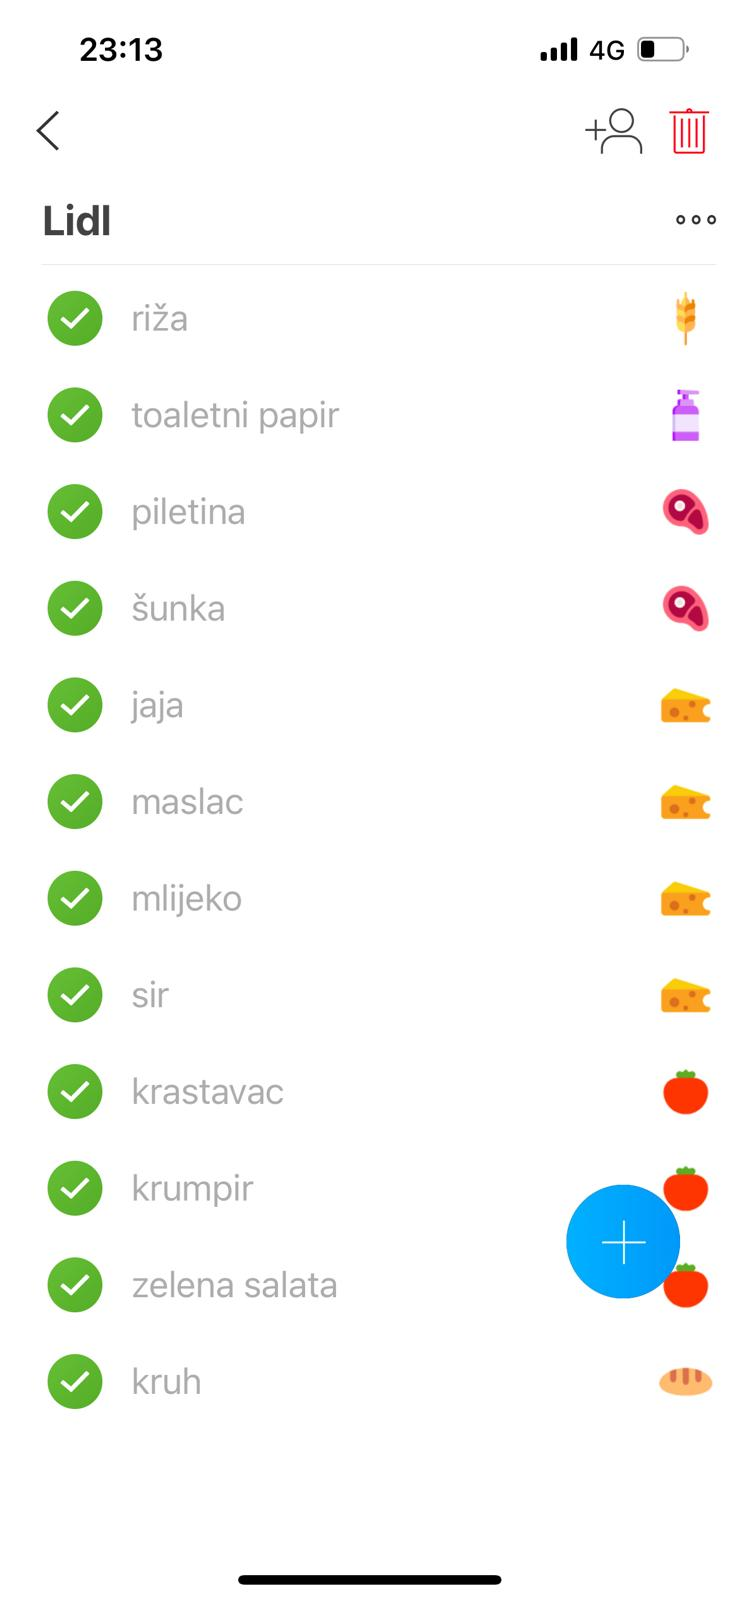
\includegraphics[width = \linewidth]{slike/listonic_primjer.JPEG}
			\centering
			\caption{Listonic}
			\label{fig:listonic}
			\end{minipage}\hfill
			\begin{minipage}[t]{0.4\linewidth}
			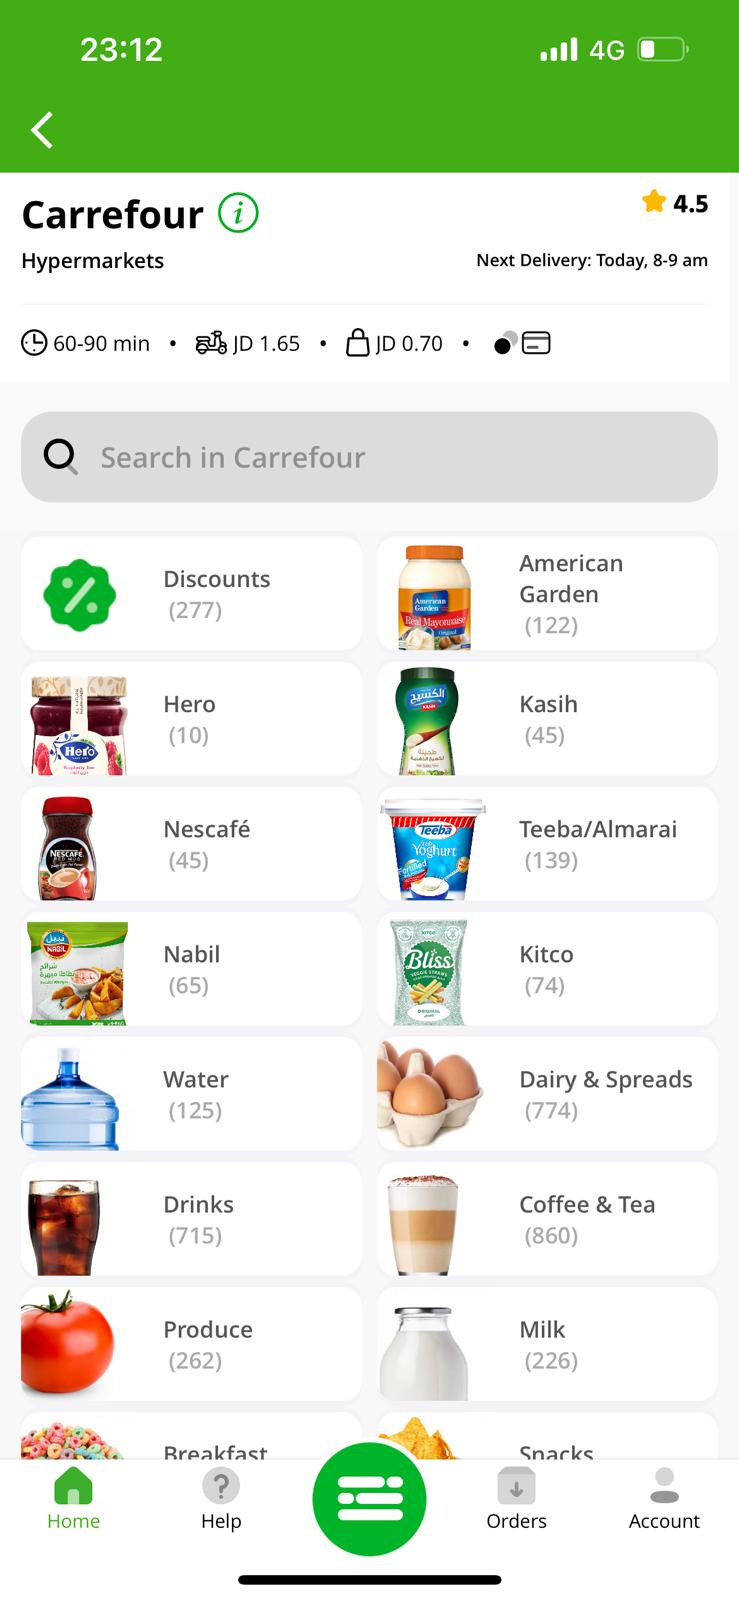
\includegraphics[width = \linewidth]{slike/basket_primjer.JPEG}
			\caption{Basket}
			\label{fig:basket}
			\end{minipage}
		\end{figure}


		\eject
		
		
		%\section{Primjeri u \LaTeX u}
		
		%\textit{Ovo potpoglavlje izbrisati.}\\

		%U nastavku se nalaze različiti primjeri kako koristiti osnovne funkcionalnosti \LaTeX a koje su potrebne za izradu dokumentacije. Za dodatnu pomoć obratiti se asistentu na projektu ili potražiti upute na sljedećim web sjedištima:
		%\begin{itemize}
		%	\item Upute za izradu diplomskog rada u \LaTeX u - \url{https://www.fer.unizg.hr/_download/repository/LaTeX-upute.pdf}
			%\item \LaTeX\ projekt - \url{https://www.latex-project.org/help/}
			%\item StackExchange za Tex - \url{https://tex.stackexchange.com/}\\
		
		%\end{itemize} 	


		
		%\noindent \underbar{podcrtani tekst}, \textbf{podebljani tekst}, 	\textit{nagnuti tekst}\\
		%\noindent \normalsize primjer \large primjer \Large primjer \LARGE {primjer} \huge {primjer} \Huge primjer \normalsize
				
		%\begin{packed_item}
			
		%	\item  primjer
		%	\item  primjer
		%	\item  primjer
		%	\item[] \begin{packed_enum}
		%		\item primjer
		%		\item[] \begin{packed_enum}
		%			\item[1.a] primjer
		%			\item[b] primjer
		%		\end{packed_enum}
		%		\item primjer
		%	\end{packed_enum}
			
		%\end{packed_item}
		
		%\noindent primjer url-a: \url{https://www.fer.unizg.hr/predmet/proinz/projekt}
		
	%	\noindent posebni znakovi: \# \$ \% \& \{ \} \_ 
	%	$|$ $<$ $>$ 
	%	\^{} 
	%	\~{} 
	%	$\backslash$ 
		
		
	%	\begin{longtblr}[
	%		label=none,
	%		entry=none
	%		]{
	%			width = \textwidth,
	%			colspec={|X[8,l]|X[8, l]|X[16, l]|}, 
	%			rowhead = 1,
	%		} %definicija širine tablice, širine stupaca, poravnanje i broja redaka naslova tablice
	%		\hline \multicolumn{3}{|c|}{\textbf{naslov unutar tablice}}	 \\ \hline[3pt]
	%		\SetCell{LightGreen}IDKorisnik & INT	&  	Lorem ipsum dolor sit amet, consectetur adipiscing elit, sed do eiusmod  	\\ \hline
	%		korisnickoIme	& VARCHAR &   	\\ \hline 
	%		email & VARCHAR &   \\ \hline 
	%		ime & VARCHAR	&  		\\ \hline 
	%		\SetCell{LightBlue} primjer	& VARCHAR &   	\\ \hline 
	%	\end{longtblr}
		

	%	\begin{longtblr}[
	%			caption = {Naslov s referencom izvan tablice},
	%			entry = {Short Caption},
	%		]{
	%			width = \textwidth, 
	%			colspec = {|X[8,l]|X[8,l]|X[16,l]|}, 
	%			rowhead = 1,
	%		}
	%		\hline
	%		\SetCell{LightGreen}IDKorisnik & INT	&  	Lorem ipsum dolor sit amet, consectetur adipiscing elit, sed do eiusmod  	\\ \hline
	%		korisnickoIme	& VARCHAR &   	\\ \hline 
	%		email & VARCHAR &   \\ \hline 
	%		ime & VARCHAR	&  		\\ \hline 
	%		\SetCell{LightBlue} primjer	& VARCHAR &   	\\ \hline 
	%	\end{longtblr}
	


		
		
		%unos slike
	%	\begin{figure}[H]
	%		\includegraphics[scale=0.4]{slike/aktivnost.PNG} %veličina slike u odnosu na originalnu datoteku i pozicija slike
	%		\centering
	%		\caption{Primjer slike s potpisom}
	%		\label{fig:promjene}
	%	\end{figure}
		
	%	\begin{figure}[H]
	%		\includegraphics[width=\textwidth]{slike/aktivnost.PNG} %veličina u odnosu na širinu linije
	%		\caption{Primjer slike s potpisom 2}
	%		\label{fig:promjene2} %label mora biti drugaciji za svaku sliku
	%	\end{figure}
		
	%	Referenciranje slike \ref{fig:promjene2} u tekstu.
		
	%	\eject
		
	

	\chapter{Specifikacija programske potpore}
		
	\section{Funkcionalni zahtjevi}
			
			%\textbf{\textit{dio 1. revizije}}\\
			
			%\textit{Navesti \textbf{dionike} koji imaju \textbf{interes u ovom sustavu} ili  \textbf{su nositelji odgovornosti}. To su prije svega korisnici, ali i administratori sustava, naručitelji, razvojni tim.}\\
				
			%\textit{Navesti \textbf{aktore} koji izravno \textbf{koriste} ili \textbf{komuniciraju sa sustavom}. Oni mogu imati inicijatorsku ulogu, tj. započinju određene procese u sustavu ili samo sudioničku ulogu, tj. obavljaju određeni posao. Za svakog aktora navesti funkcionalne zahtjeve koji se na njega odnose.}\\
			
			
			\noindent \textbf{Dionici:}
			 
			\begin{packed_enum}
				
				\item Neregistrirani korisnik
				\item Registrirani korisnik				
				\item Administrator
                \item Trgovina\\
				
			\end{packed_enum}
   
			
			\noindent \textbf{Aktori i njihovi funkcionalni zahtjevi:}
			
			
			\begin{packed_enum}
				\item  \underbar{Neregistrirani korisnik (inicijator) može:}
				
				\begin{enumerate}
					
					\item pregledavati sadržaj aplikacije
					\item se registrirati u sustav, stvoriti novi korisnički račun za koji su mu potrebni korisničko ime, prezime, nadimak i e-mail
			
					
				\end{enumerate}
			
				\item  \underbar{Registrirani korisnik (sudionik) može:}
				
				\begin{enumerate}
					
					\item birati što od navedenog će biti javno, a što privatno
					\item pregledavati sadržaj aplikacije
        	        \item unositi cijene i dodavati oznake proizvodima
                        \item predložiti oznaku za proivod
                        
					
				\end{enumerate}

                \item  \underbar{Administrator (sudionik) može:}
				
				\begin{enumerate}
					
					\item birati što od navedenog će biti javno, a što privatno
					\item pregledavati sadržaj aplikacije
        	        \item unositi cijene i dodavati oznake proizvodima
                        \item zabraniti pristup stranici registriranim korisnicima ili trgovinama
                        \item napisati komentar o svakoj pojedinoj trgovini koji je istaknut na stranici trgovine
                        
					
				\end{enumerate}

                \item  \underbar{Trgovina (sudionik) može:}
				
				\begin{enumerate}
					
					\item se registrirati u sustav, te prilikom registracije mora unijeti popis svih svojih proizvoda i njihove standardne cijene
					\item svaki dan na svoje računalo postaviti datoteku u kojoj se nalaze cijene onih proizvoda koje odstupaju od standardnih
        	        
                        
					
				\end{enumerate}

    
			\end{packed_enum}
			
			\eject 
			
			
				
			\subsection{Obrasci uporabe}
				
				%\textbf{\textit{dio 1. revizije}}
				
				%\subsubsection{Opis obrazaca uporabe}
				%	\textit{Funkcionalne zahtjeve razraditi u obliku obrazaca uporabe. Svaki obrazac je potrebno razraditi prema donjem predlošku. Ukoliko u nekom koraku može doći do odstupanja, potrebno je to odstupanje opisati i po mogućnosti ponuditi rješenje kojim bi se tijek obrasca vratio na osnovni tijek.}\\
					

					%\noindent \underbar{\textbf{UC$<$broj obrasca$>$ -$<$ime obrasca$>$}}
					%\begin{packed_item}
	
					%	\item \textbf{Glavni sudionik: }$<$sudionik$>$
					%	\item  \textbf{Cilj:} $<$cilj$>$
					%	\item  \textbf{Sudionici:} $<$sudionici$>$
					%	\item  \textbf{Preduvjet:} $<$preduvjet$>$
					%	\item  \textbf{Opis osnovnog tijeka:}
						
					%	\item[] \begin{packed_enum}
	
					%		\item $<$opis korak jedan$>$
					%		\item $<$opis korak dva$>$
					%		\item $<$opis korak tri$>$
					%		\item $<$opis korak četiri$>$
					%		\item $<$opis korak pet$>$
					%	\end{packed_enum}
						
					%	\item  \textbf{Opis mogućih odstupanja:}
						
					%	\item[] \begin{packed_item}
	
					%		\item[2.a] $<$opis mogućeg scenarija odstupanja u koraku 2$>$
					%		\item[] \begin{packed_enum}
								
					%			\item $<$opis rješenja mogućeg scenarija korak 1$>$
					%			\item $<$opis rješenja mogućeg scenarija korak 2$>$
								
					%		\end{packed_enum}
					%		\item[2.b] $<$opis mogućeg scenarija odstupanja u koraku 2$>$
					%		\item[3.a] $<$opis mogućeg scenarija odstupanja  u koraku 3$>$\\
							
					%	\end{packed_item}
					%\end{packed_item}

                        \noindent \underbar{\textbf{UC1 - Pregled sadržaja}}
					\begin{itemize}
	
						\item \textbf{Glavni sudionik: }Korisnik
						\item  \textbf{Cilj:} Pregledati proizvode i ponude
						\item  \textbf{Sudionici:} Baza podataka
						\item  \textbf{Preduvjet:} -
						\item  \textbf{Opis osnovnog tijeka:}
						
						\item[] \begin{enumerate}
							\item Prilikom učitavanja aplikacije prikazuje se ponuda\\
						\end{enumerate}
						
					\end{itemize}


                        \noindent \underbar{\textbf{UC2 - Registracija}}
					\begin{itemize}
	
						\item \textbf{Glavni sudionik: }Korisnik
						\item  \textbf{Cilj:} Stvoriti korisnički račun za pristup sustavu
						\item  \textbf{Sudionici:} Baza podataka
						\item  \textbf{Preduvjet:} -
						\item  \textbf{Opis osnovnog tijeka:}
						
						\item[] \begin{enumerate}
							\item Korisnik odabire opciju za registraciju
                                \item Korisnik unosi potrebne korisničke podatke
                                \item Korisnik prima obavijest o uspješnoj registraciji
						\end{enumerate}

                            \item  \textbf{Opis mogućih odstupanja:}
						
						\item[] \begin{enumerate}
	
							\item[2.a] Odabir već zauzetog korisničkog imena i/ili e-maila, unos korisničkog podatka u nedozvoljenom formatu ili pružanje neispravnog e-maila
							\item[] \begin{enumerate}
								
								\item Sustav obavještava korisnika o neuspjelom upisu i vraća ga na stranicu za registraciju
								\item Korisnik mijenja potrebne podatke te završava unos ili odustaje od registracije\\
								
							\end{enumerate}
			
							
						\end{enumerate}
						
					\end{itemize}

                        \noindent \underbar{\textbf{UC3 - Prijava u sustav}}
					\begin{itemize}
	
						\item \textbf{Glavni sudionik: }Korisnik
						\item  \textbf{Cilj:} Dobiti pristup korisničkom sučelju
						\item  \textbf{Sudionici:} Baza podataka
						\item  \textbf{Preduvjet:} Registracija
						\item  \textbf{Opis osnovnog tijeka:}
						
						\item[] \begin{enumerate}
							\item Unos korisničkog imena i lozinke
                                \item Potvrda o ispravnosti unesenih podataka
                                \item Pristup korisničkim funkcijama
						\end{enumerate}

                            \item  \textbf{Opis mogućih odstupanja:}
						
						\item[] \begin{enumerate}
	
							\item[2.a] Neispravno korisničko ime/lozinka
							\item[] \begin{enumerate}
								
								\item Sustav obavještava korisnika o neuspjelom upisu i vraća ga na stranicu za prijavu\\
								
							\end{enumerate}
			
							
						\end{enumerate}
						
					\end{itemize}

                        \noindent \underbar{\textbf{UC4 - Pregled osobnih podataka}}
					\begin{itemize}
	
						\item \textbf{Glavni sudionik: }Korisnik
						\item  \textbf{Cilj:} Pregledati osobne podatke
						\item  \textbf{Sudionici:} Baza podataka
						\item  \textbf{Preduvjet:} Korisnik je prijavljen
						\item  \textbf{Opis osnovnog tijeka:}
						
						\item[] \begin{enumerate}
							\item Korisnik odabire opciju "Osobni podatci"
                                \item Aplikacija prikazuje osobne podatke korisnika\\
						\end{enumerate}
			
						
					\end{itemize}

                        \noindent \underbar{\textbf{UC5 - Promjena osobnih podataka}}
					\begin{itemize}
	
						\item \textbf{Glavni sudionik: }Korisnik
						\item  \textbf{Cilj:} Promijeniti osobne podatke
						\item  \textbf{Sudionici:} Baza podataka
						\item  \textbf{Preduvjet:} Korisnik je prijavljen
						\item  \textbf{Opis osnovnog tijeka:}
						
						\item[] \begin{enumerate}
							\item Korisnik odabire opciju za promjenu podataka
                                \item Korisnik mijenja svoje osobne podatke
                                \item Korisnik sprema promjene
                                \item Baza podataka se ažurira
						\end{enumerate}

                            \item  \textbf{Opis mogućih odstupanja:}
						
						\item[] \begin{enumerate}
	
							\item[2.a] Korisnik mijenja svoje podatke, ali ne odabire opciju "Spremi promjenu"
							\item[] \begin{enumerate}
								
								\item Sustav obavještava korisnika o neuspjeloj promjeni podataka prije izlaska iz prozora\\
								
							\end{enumerate}
			
							
						\end{enumerate}
						
					\end{itemize}


                        \noindent \underbar{\textbf{UC6 - Brisanje korisničkog računa}}
					\begin{itemize}
	
						\item \textbf{Glavni sudionik: }Korisnik
						\item  \textbf{Cilj:} Izbrisati svoj korisnički račun
						\item  \textbf{Sudionici:} Baza podataka
						\item  \textbf{Preduvjet:} Korisnik je prijavljen
						\item  \textbf{Opis osnovnog tijeka:}
						
						\item[] \begin{enumerate}
							\item Korisnik pregledava osobne podatke
                                \item Otvara se stranica s osobnim podatcima korisnika
                                \item Korisnik briše račun
                                \item Baza podataka se ažurira tj. korisnički račun se izbriše iz baze podataka
                                \item Otvara se stranica za registraciju\\
						\end{enumerate}
						
					\end{itemize}

                        \noindent \underbar{\textbf{UC7 - Unos cijena proizvoda}}
					\begin{itemize}
	
						\item \textbf{Glavni sudionik: }Korisnik
						\item  \textbf{Cilj:} Unijeti cijene proizvoda koje odstupaju od onih na aplikaciji
						\item  \textbf{Sudionici:} Baza podataka
						\item  \textbf{Preduvjet:} Korisnik je prijavljen
						\item  \textbf{Opis osnovnog tijeka:}
						
						\item[] \begin{enumerate}
							\item Korisnik odabire trgovinu u kojoj je zapazio drugačiju cijenu
                                \item Korisnik unosi novu cijenu
                                \item Korisnik prilaže sliku na kojoj je vidljiva cijena u navedenoj trgovini
                                \item Zahtjev se šalje administratoru na provjeru\\
						\end{enumerate}
						
					\end{itemize}


                        \noindent \underbar{\textbf{UC8 - Provjera promjene cijene}}
					\begin{itemize}
	
						\item \textbf{Glavni sudionik: }Administrator
						\item  \textbf{Cilj:} Potvrditi promjenu cijene 
						\item  \textbf{Sudionici:} Baza podataka
						\item  \textbf{Preduvjet:} Korisnik je prijavljen i dodijeljena su mu prava administratora
						\item  \textbf{Opis osnovnog tijeka:}
						
						\item[] \begin{enumerate}
							\item Administrator odabire opciju za pregled zahtjeva
                                \item Administrator odabire zahtjev
                                \item Administrator provjerava zahtjev i odobrava ga
                                \item Šalje obavijest o promijeni cijene korisniku i trgovini
						\end{enumerate}

                            \item  \textbf{Opis mogućih odstupanja:}
						
						\item[] \begin{enumerate}
	
							\item[3.a] Korisnik unosi cijenu koja je jednaka cijeni na aplikaciji
							\item[] \begin{enumerate}
								\item Administrator odbija zahtjev
								\item Sustav šalje obavijest korisniku o neuspjeloj promijeni cijene\\
								
							\end{enumerate}
			
							
						\end{enumerate}
						
					\end{itemize}

                        \noindent \underbar{\textbf{UC9 - Promjena prava pristupa}}
					\begin{itemize}
	
						\item \textbf{Glavni sudionik: }Administrator
						\item  \textbf{Cilj:} Promijeniti razinu pristupa korisnika ili trgovine
						\item  \textbf{Sudionici:} Baza podataka
						\item  \textbf{Preduvjet:} Korisnik je prijavljen i dodijeljena su mu prava administratora
						\item  \textbf{Opis osnovnog tijeka:}
						
						\item[] \begin{enumerate}
							\item Administrator odabire opciju za promjenu prava pristupa
                                \item Administrator pronalazi željenog korisnika ili trgovinu
                                \item Administrator mijenja razinu pristupa željenom korisniku\\
						\end{enumerate}

					\end{itemize}


                        \noindent \underbar{\textbf{UC10 - Dodavanje komentara trgovinama}}
					\begin{itemize}
	
						\item \textbf{Glavni sudionik: }Administrator
						\item  \textbf{Cilj:} Dodati komentar određenoj trgovini
						\item  \textbf{Sudionici:} Baza podataka
						\item  \textbf{Preduvjet:} Korisnik je prijavljen i dodijeljena su mu prava administratora
						\item  \textbf{Opis osnovnog tijeka:}
						
						\item[] \begin{enumerate}
							\item Administrator odabire opciju za dodavanje komentara trgovini
                                \item Administrator pronalazi željenu trgovinu
                                \item Administrator dodaje komentar\\
						\end{enumerate}

					\end{itemize}


                        \noindent \underbar{\textbf{UC11 - Dodavanje oznaka proizvodima}}
					\begin{itemize}
	
						\item \textbf{Glavni sudionik: }Korisnik
						\item  \textbf{Cilj:} Dodati oznaku određenom proizvodu
						\item  \textbf{Sudionici:} Baza podataka
						\item  \textbf{Preduvjet:} Korisnik je prijavljen
						\item  \textbf{Opis osnovnog tijeka:}
						
						\item[] \begin{enumerate}
							\item Korisnik odabire proizvod
                                \item Korisnik bira oznaku za odabrani proizvod\\
						\end{enumerate}

					\end{itemize}

                        \noindent \underbar{\textbf{UC12 - Registracija trgovine}}
					\begin{itemize}
	
						\item \textbf{Glavni sudionik: }Trgovina
						\item  \textbf{Cilj:} Stvoriti račun za trgovinu kako bi pristupila sustavu
						\item  \textbf{Sudionici:} Baza podataka
						\item  \textbf{Preduvjet:} -
						\item  \textbf{Opis osnovnog tijeka:}
						
						\item[] \begin{enumerate}
							\item Trgovina odabire opciju za registraciju trgovine
                                \item Trgovina unosi potrebne podatke za registraciju trgovine
                                \item Trgovina unosi popis svih proizvoda i njihove standardne cijene
                                \item Trgovina prima obavijest o uspješnoj registraciji trgovine
						\end{enumerate}

                            \item  \textbf{Opis mogućih odstupanja:}
						
						\item[] \begin{enumerate}
	
							\item[2.a] Odabir već zauzetog imena trgovine i/ili e-maila, unos podatka u nedozvoljenom formatu
							\item[] \begin{enumerate}
								
								\item Sustav obavještava trgovinu o neuspjelom upisu i vraća ga na stranicu za registraciju trgovine
								\item Trgovina mijenja potrebne podatke te završava unos ili odustaje od registracije\\
								
							\end{enumerate}
			
							
						\end{enumerate}
						
					\end{itemize}

                        \noindent \underbar{\textbf{UC13 - Prijava trgovine u sustav}}
					\begin{itemize}
	
						\item \textbf{Glavni sudionik: }Trgovina
						\item  \textbf{Cilj:}  Trgovini omogućiti pristup sučelju
						\item  \textbf{Sudionici:} Baza podataka
						\item  \textbf{Preduvjet:} Registracija trgovine
						\item  \textbf{Opis osnovnog tijeka:}
						
						\item[] \begin{enumerate}
							\item Unos imena trgovine i lozinke
                                \item Potvrda o ispravnosti unesenih podataka
                                \item Pristup funkcijama trgovina
						\end{enumerate}

                            \item  \textbf{Opis mogućih odstupanja:}
						
						\item[] \begin{enumerate}
	
							\item[2.a] Neispravno ime trgovine/lozinka
							\item[] \begin{enumerate}
								
								\item Sustav obavještava trgovinu o neuspjelom upisu i vraća ju na stranicu za prijavu trgovine\\
								
							\end{enumerate}
			
							
						\end{enumerate}
						
					\end{itemize}

                        \noindent \underbar{\textbf{UC14 - Postavljanje datoteke s novim cijenama}}
					\begin{itemize}
	
						\item \textbf{Glavni sudionik: }Trgovina
						\item  \textbf{Cilj:} Postaviti nove cijene proizvoda
						\item  \textbf{Sudionici:} Baza podataka
						\item  \textbf{Preduvjet:} Registracija trgovine
						\item  \textbf{Opis osnovnog tijeka:}
						
						\item[] \begin{enumerate}
							\item Trgovina postavlja datoteku na računalo 
                                \item Web-aplikacija dohvaća postavljenu datoteku i ažurira bazu podataka
						\end{enumerate}

                            \item  \textbf{Opis mogućih odstupanja:}
						
						\item[] \begin{enumerate}
	
							\item[2.a] Trgovina nije priložila datoteku
							\item[] \begin{enumerate}
								
								\item Sustav pretpostavlja da nema promjena u cijenama\\
								
							\end{enumerate}
							\item[2.b] Trgovina je priložila neispravnu datoteku
							\item[] \begin{enumerate}
								\item Sustav šalje poruku trgovini o neispravnoj datoteci
							\end{enumerate}
			
							
						\end{enumerate}
						
					\end{itemize}
					
					
					\noindent \underbar{\textbf{UC15 - Određivanje javno/privatno}}
					\begin{itemize}
	
						\item \textbf{Glavni sudionik: }Korisnik
						\item  \textbf{Cilj:} Promijeniti vidljivost svojih podataka (javno/privatno)
						\item  \textbf{Sudionici:} Baza podataka
						\item  \textbf{Preduvjet:} Korisnik je prijavljen
						\item  \textbf{Opis osnovnog tijeka:}
						
						\item[] \begin{enumerate}
							\item Korisnik odabire opciju za uređivanje osobnog profila
                                \item Korisnik odlučuje što će biti javno. a što dostupno privatno\\
						\end{enumerate}

					\end{itemize}

                    

                        


     
					
				\subsubsection{Dijagrami obrazaca uporabe}
					
					%\textit{Prikazati odnos aktora i obrazaca uporabe odgovarajućim UML dijagramom. Nije nužno nacrtati sve na jednom dijagramu. Modelirati po razinama apstrakcije i skupovima srodnih funkcionalnosti.}
					\begin{figure}[H]
			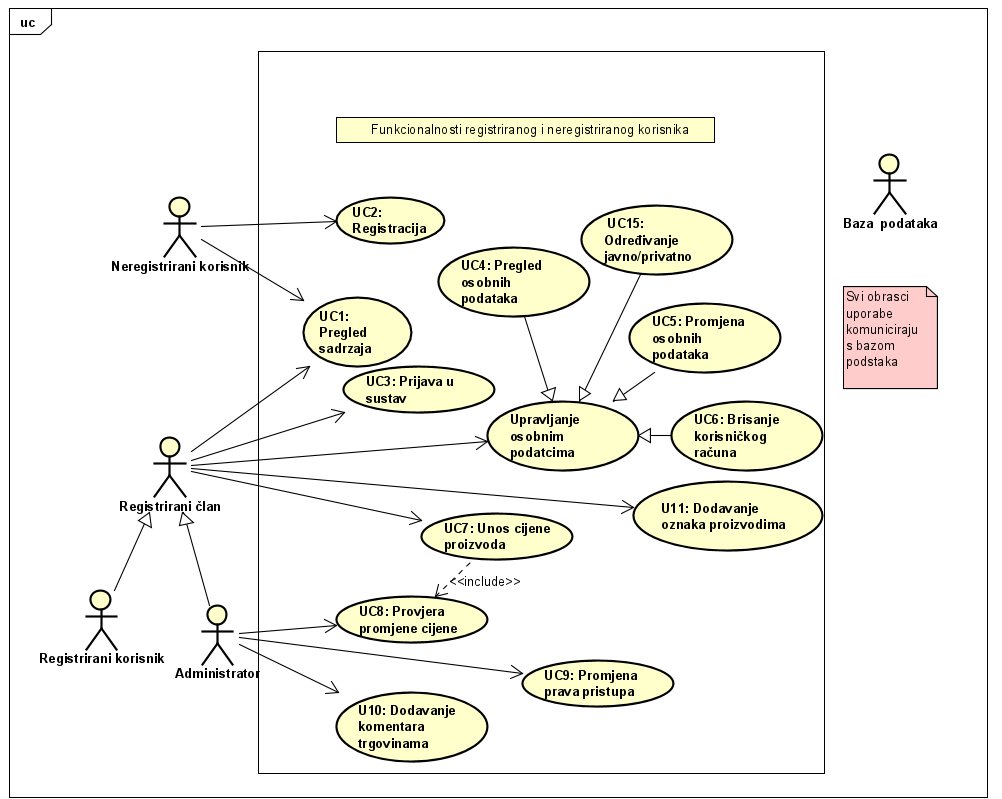
\includegraphics[width=\textwidth]{slike/Korisnik.PNG} %veličina u odnosu na širinu linije
			\caption{Use case dijagram - Korisnik}
			\label{fig:Korisnik} %label mora biti drugaciji za svaku sliku
			\end{figure}
			
			\begin{figure}[H]
			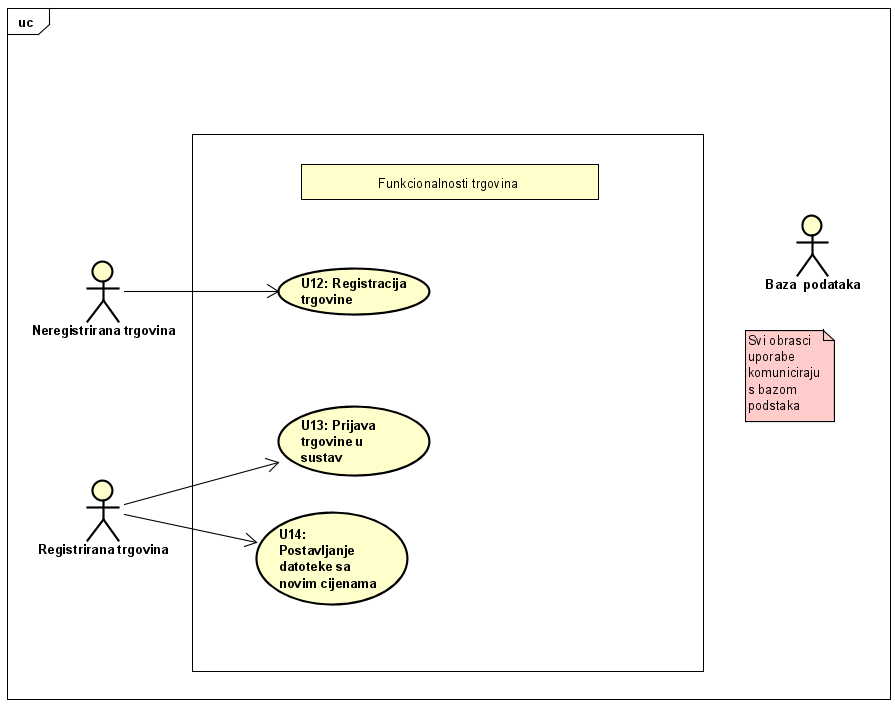
\includegraphics[width=\textwidth]{slike/Trgovina.PNG} %veličina u odnosu na širinu linije
			\caption{Use case dijagram - Trgovina}
			\label{fig:Trgovina} %label mora biti drugaciji za svaku sliku
			\end{figure}
				\eject		
				
			\subsection{Sekvencijski dijagrami}
				
				%\textbf{\textit{dio 1. revizije}}\\
				
				%\textit{Nacrtati sekvencijske dijagrame koji modeliraju najvažnije dijelove sustava (max. 4 dijagrama). Ukoliko postoji nedoumica oko odabira, razjasniti s asistentom. Uz svaki dijagram napisati detaljni opis dijagrama.}
				\underline{\textbf{UC2 - Registracija}}\\
				
				Neregistrirani korisnik želi se registrirati kako bi dobio pogodnosti registriranog korisnika. Kako bi to učinio prvu odabire opciju za registraciju nakon koje mu se pokazuje register page. Unosi korisničke podatke u predviđena polja (e-mail, korisničko ime, ime, prezime i lozinku.) Aplikacija zatim provjerava s bazom postoje li profili s tom e-mail adresom ili tim korisničkim imenom. Ako su e-mail i/ili korisničko ime zauzeti, aplikacija dojavljuje pogrešku, vraća ga na stranicu za registraciju te prikazuje obavijest da izabere neku drugu e-mail adresu ili korisničko ime. Korisnik može isprobavati slobodne opcije sve dok jedna kombinacija ne bude jedinstvena ili može odustati od registracije. Kada korisnik unese jedinstvenu kombinaciju e-maila i korisničkog imena, uspješno se registrira i sustav mu šalje obavijest o uspješnoj registraciji.
				
			\begin{figure}[H]
			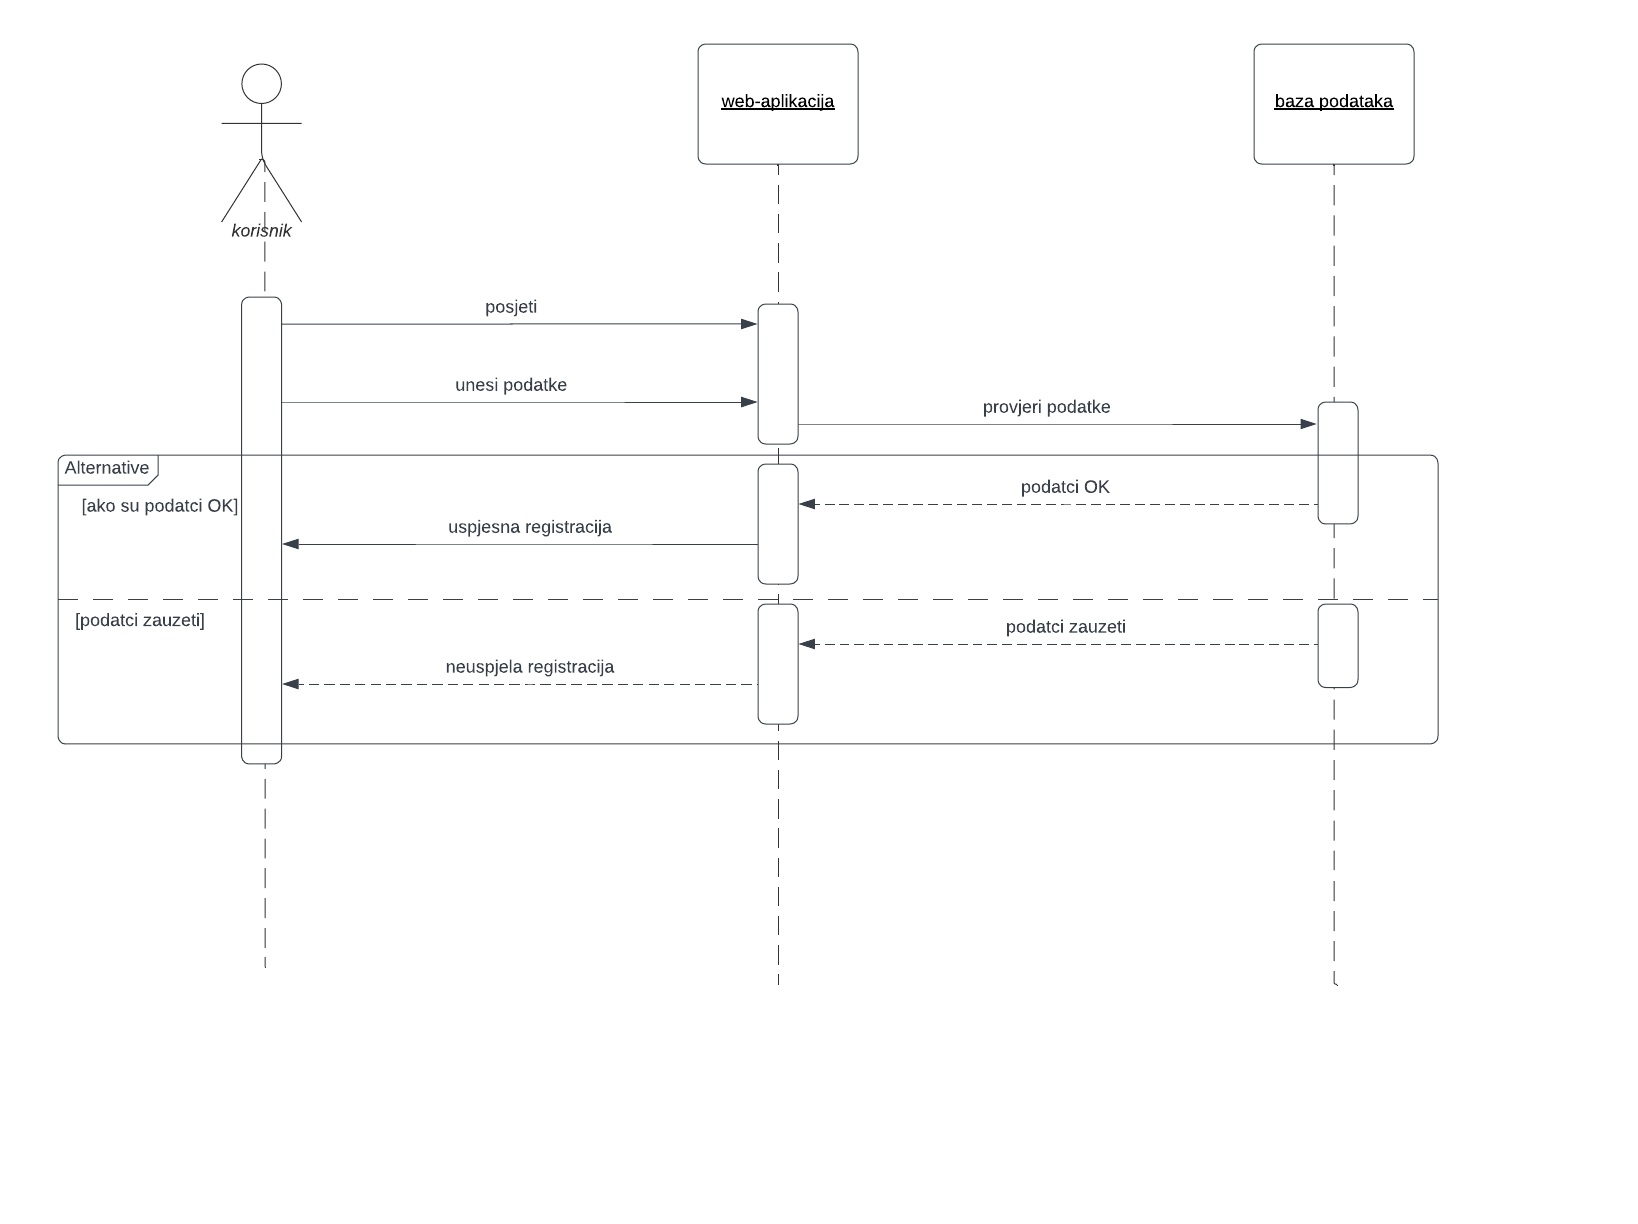
\includegraphics[width=\textwidth]{slike/uc2.PNG} %veličina u odnosu na širinu linije
			\caption{UC2 - sekvencijski dijagram}
			\label{fig:promjene2} %label mora biti drugaciji za svaku sliku
			\end{figure}
				
				\underline{\textbf{UC7 - Unos cijene proizvoda, UC8 - Provjera promjene cijene}}\\
				
				Ako postoji razlika u cijenama u trgovini i na web-stranici, korisnik odabire trgovinu u kojoj je zapazio drugačiju cijenu, unosi novu cijenu, šalje sliku proizvoda i stvarne cijene u aplikaciju. Aplikacija tu sliku sprema u bazu podataka odakle administrator odabire opciju za pregled zahtjeva, odabire zahtjev te preuzima sliku na pregled. Ako su slike u redu, administrator šalje potvrdu, cijena se promijeni te se pošalje poruka potvrde korisniku i trgovini. Ako se cijene ne podudaraju ili je zahtjev neispravan, administrator odbija zahtjev i sustav šalje obavijest korisniku o neuspjeloj promjeni cijene.
				
				\begin{figure}[H]
			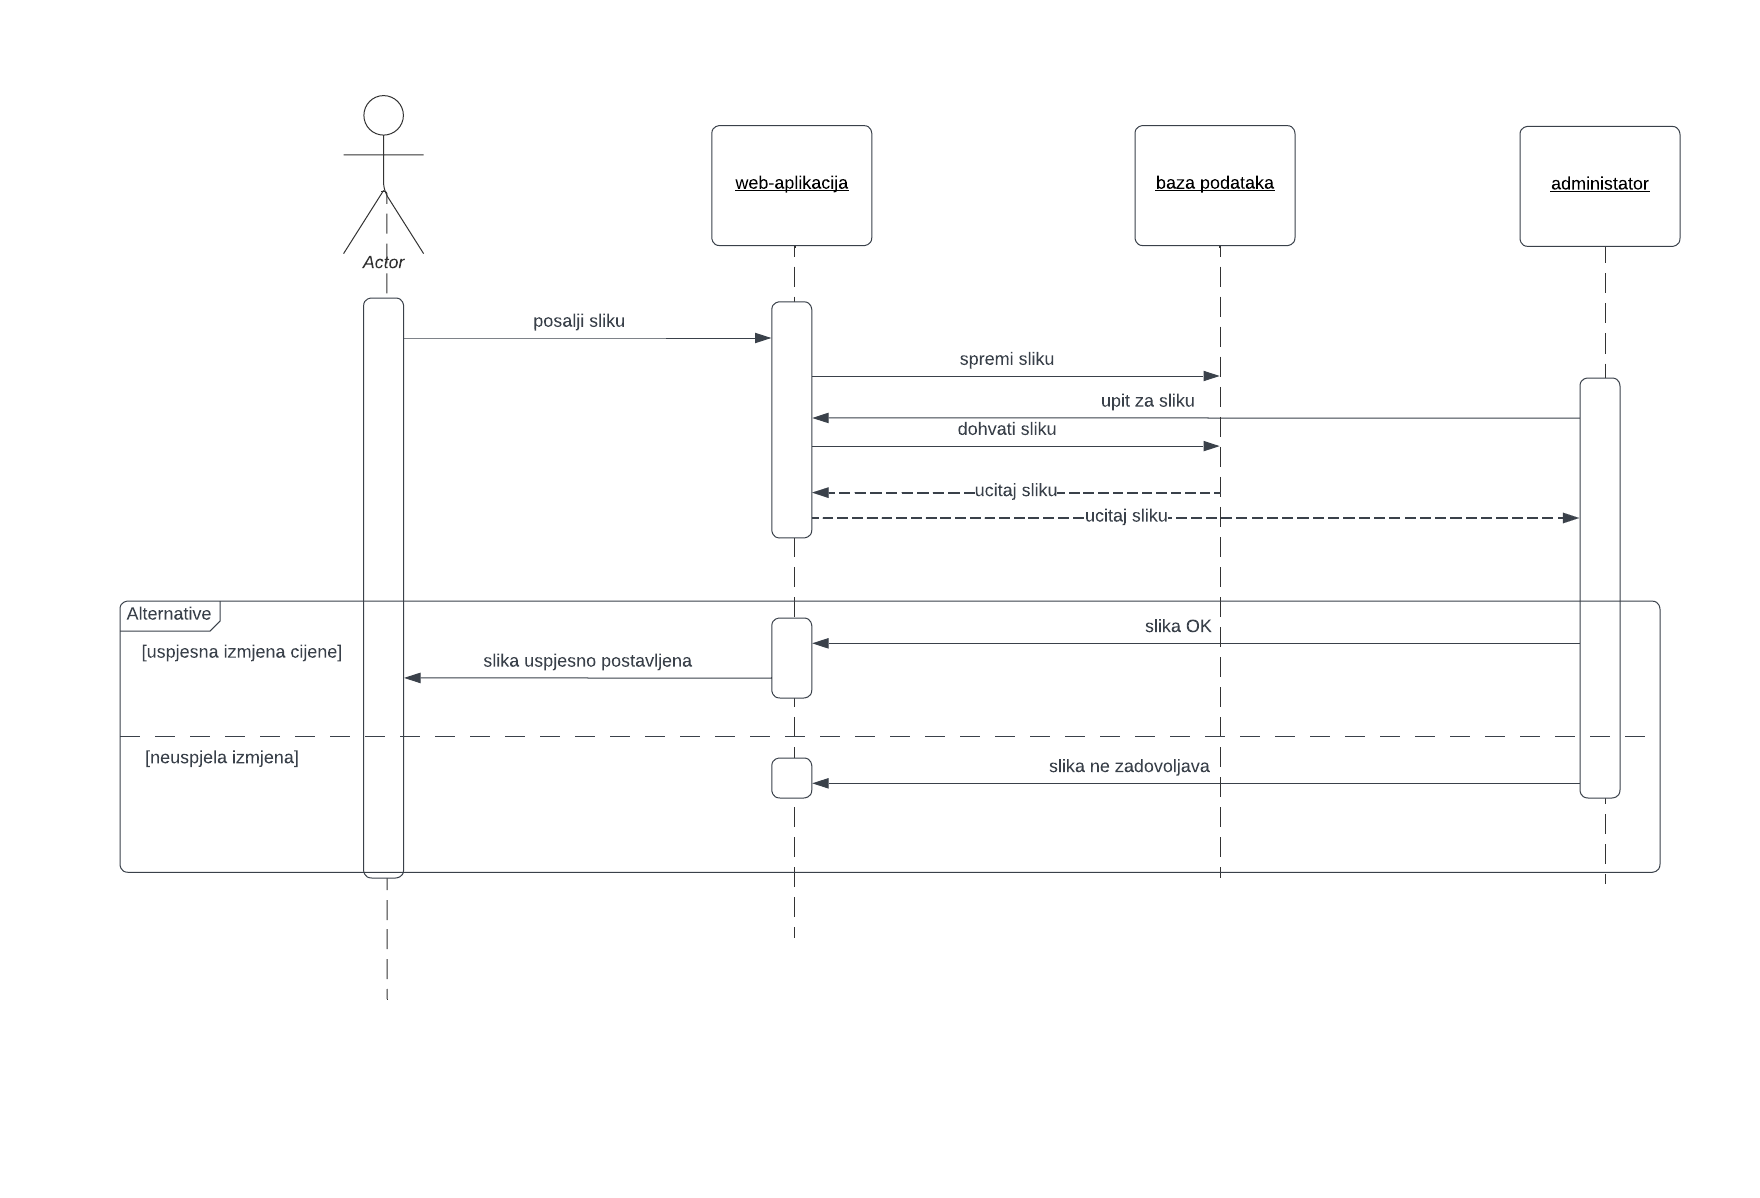
\includegraphics[width=\textwidth]{slike/uc7_cropped.PNG} %veličina u odnosu na širinu linije
			\caption{UC7, UC8 - sekvencijski dijagram}
			\label{fig:promjene2} %label mora biti drugaciji za svaku sliku
			\end{figure}
			
			\underline{\textbf{UC14 - Postavljanje datoteke sa novim cijenama}}\\
				
				Početkom svakog radnog dana trgovina unosi datoteku s promjenama cijena na svoje računalo. Web-aplikacija automatski preuzima tu datoteku i ažurira cijene u bazi podataka. Ako trgovina nije postavila datoteku, podrazumijeva se da nema promjena. Ako trgovina neispravno postavi datoteku, sustav obavještava trgovinu o neuspjeloj predaji.
				
				\begin{figure}[H]
			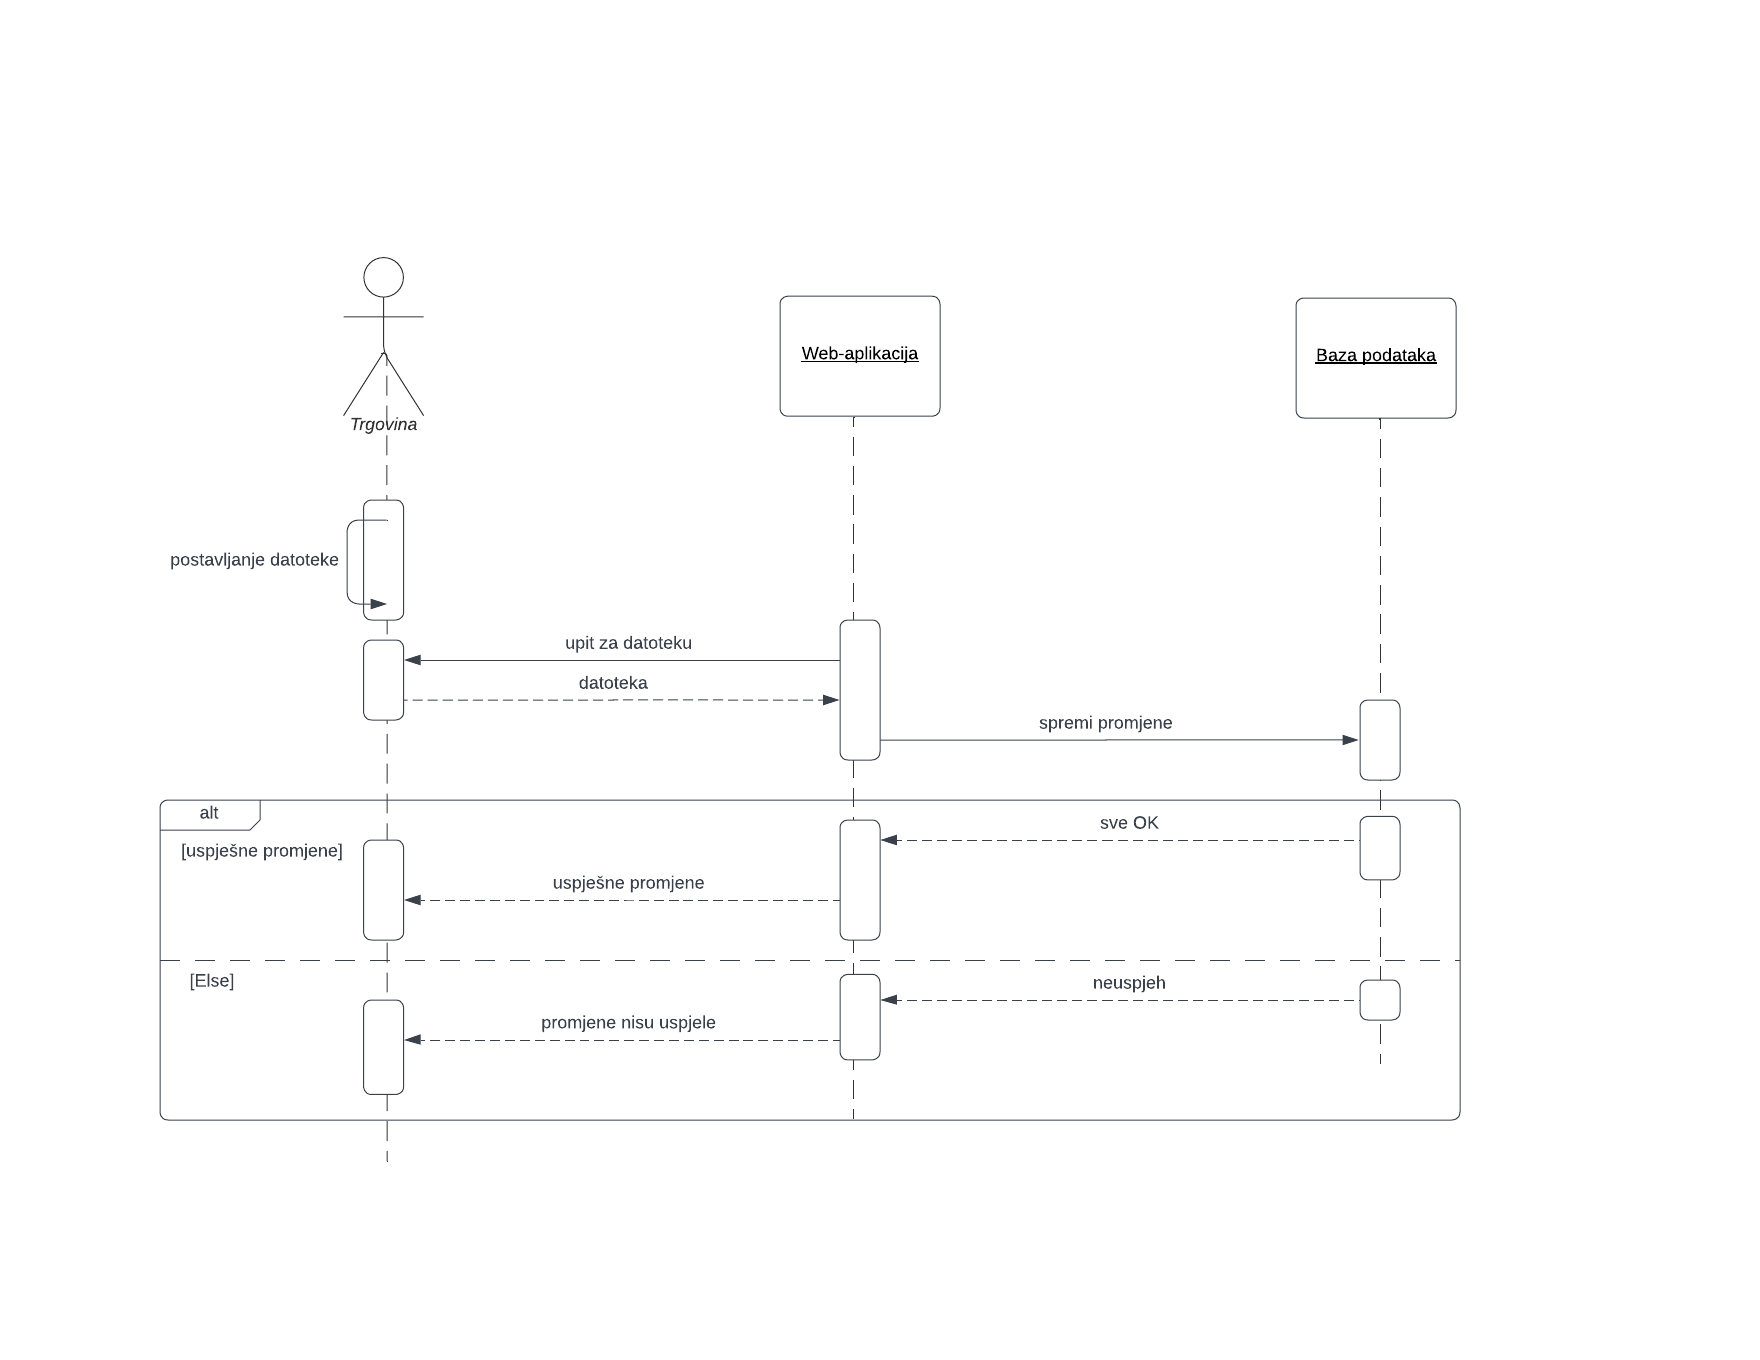
\includegraphics[width=\textwidth]{slike/uc14.PNG} %veličina u odnosu na širinu linije
			\caption{UC14 - sekvencijski dijagram}
			\label{fig:promjene2} %label mora biti drugaciji za svaku sliku
			\end{figure}
				\eject
	
		\section{Ostali zahtjevi}
		
			%\textbf{\textit{dio 1. revizije}}\\
		 
			%\textit{Nefunkcionalni zahtjevi i zahtjevi domene primjene dopunjuju funkcionalne zahtjeve. Oni opisuju \textbf{kako se sustav treba ponašati} i koja \textbf{ograničenja} treba poštivati (performanse, korisničko iskustvo, pouzdanost, standardi kvalitete, sigurnost...). Primjeri takvih zahtjeva u Vašem projektu mogu biti: podržani jezici korisničkog sučelja, vrijeme odziva, najveći mogući podržani broj korisnika, podržane web/mobilne platforme, razina zaštite (protokoli komunikacije, kriptiranje...)... Svaki takav zahtjev potrebno je navesti u jednoj ili dvije rečenice.}
			\begin{itemize}
                \item Omogućen istovremeni rad više korisnika
                \item Postupak pristupa bazi podataka ne smije trajati duže od nekoliko sekundi
                \item Sustav treba biti implementiran kao web aplikacija koristeći objektno-orijentirane jezike
                \item Funkcionalnost i rad sustava ne smiju biti narušeni neispravnim korištenjem korisničkog sučelja. 
                \item Sustav treba biti jednostavan i intuitivan za korištenje
                \item Postojeće funkcionalnosti sustava trebaju biti održane pri nadogradnji sustava
                \item Veza s bazom podataka mora biti kvalitetno zaštićena, brza i otporna na vanjske greške
                \item Pristup serveru mora biti omogućen iz javne mreže pomoću HTTPS
                \item Korisničko sučelje i sustav moraju podržavati hrvatsku abecedu (dijakritičke znakove) pri unosu i prikazu tekstualnog sadržaja
                \item Sustav kao valutu koristi EUR
            \end{itemize}
			 
			 
		
	\chapter{Arhitektura i dizajn sustava}
		
		%\textbf{\textit{dio 1. revizije}}\\

		%\textit{ Potrebno je opisati stil arhitekture te identificirati: podsustave, preslikavanje na radnu platformu, spremišta podataka, mrežne protokole, globalni upravljački tok i sklopovsko-programske zahtjeve. Po točkama razraditi i popratiti odgovarajućim skicama:}
	%\begin{itemize}
		%\item 	\textit{izbor arhitekture temeljem principa oblikovanja pokazanih na predavanjima (objasniti zašto ste baš odabrali takvu arhitekturu)}
		%\item 	\textit{organizaciju sustava s najviše razine apstrakcije (npr. klijent-poslužitelj, baza podataka, datotečni sustav, grafičko sučelje)}
		%\item 	\textit{organizaciju aplikacije (npr. slojevi frontend i backend, MVC arhitektura) }		
	%\end{itemize}

	Stil arhitekture koji smo odabrali je arhitektura zasnovana na događajima gdje se događaji javno objavljuju te se pozivaju registrirane procedure, dok komponente koje objavljuju događaj nemaju informaciju koje će sve komponente reagirati i kako. Za razliku od objektno usmjerenog stila, komponente se ne pozivaju eksplicitno, već generiraju signale, tj. događaje. Ova arhitektura je odabrana jer je najefikasnija za obradu korisničkih zahtjeva, laka je za održavanje i reciklabilna za potrebe budućih projekata ili nadogradnje ovog. Što se tiče spremišta podataka, svi podaci će biti spremani te dohvaćani iz univerzalne baze podataka. Mrežni protokoli koji će se pozivati tokom komunikacije klijenta s poslužiteljem su: TCP, IP, HTTP. 
Sustav je organiziran na sljedeći način: 
\begin{figure}[H]
			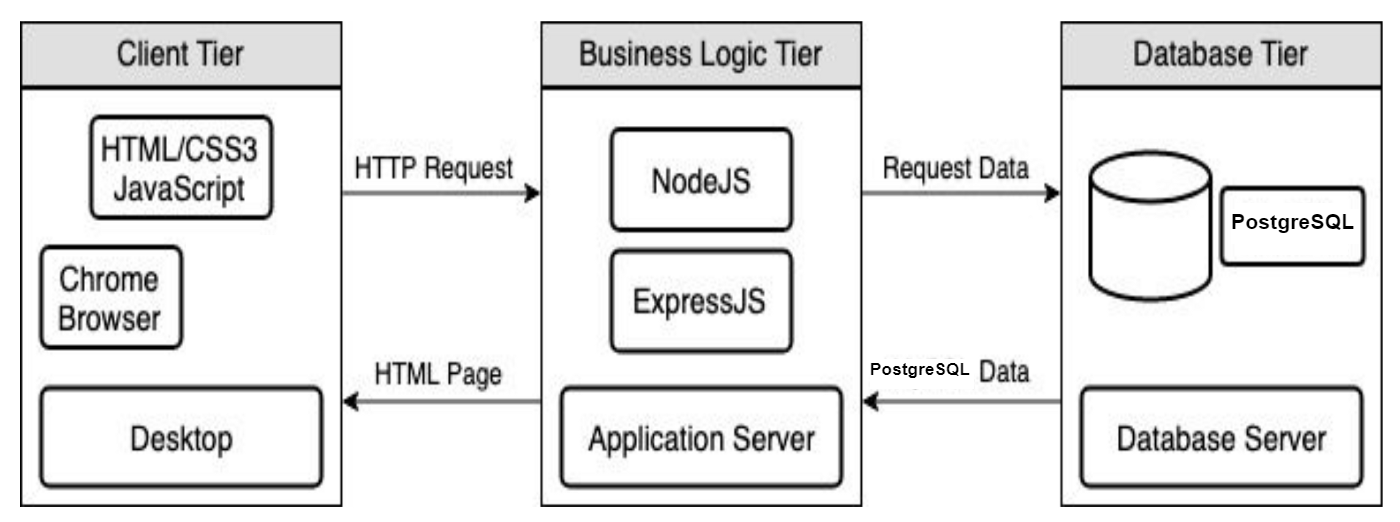
\includegraphics[width=\textwidth]{slike/arhitekturaSkica.png} %veličina u odnosu na širinu linije
			\caption{grafički prikaz arhitekture}
			\label{fig:arhitektura} %label mora biti drugaciji za svaku sliku
			\end{figure}
Korisnik putem odabranog web preglednika šalje HTTP zahtjev za web aplikacijom i njenim komponentama zadanom web poslužitelju. Aplikacija komunicira s bazom podataka u kojoj su sadržani svi podatci i iz nje izvlači sve potrebne podatke za klijentov zahtjev. Poslužitelj, kada aplikacija dohvati sve potrebne podatke, odgovara na klijentov zahtjev sa statusom 200 OK (ako je sve u redu) i šalje mu HTML dokument koji se prikazuje u zadanom web pregledniku.
Programski jezik koji smo koristili za izradu web aplikacije je Java za backend te Javascript za frontend dio.
Arhitektura sustava se temelji na MVC konceptu, stilističkoj varijaciji arhitekture zasnovanoj na događajima. Odabrali smo taj koncept jer odvaja korisničko sučelje od ostatka sustava, što čini razvoj i nadogradnju komponenata jednostavnijima. Sastoji se od modela, pogleda i upravitelja.
		
\begin{itemize}
\item Model – dojavljuje sebi pridruženim pogledima i upravitelju kada je došlo do promjene u njegovom stanju. Ove dojave omogućuju pogledu da prikaže obnovljeno stanje modela, a upravitelju promjenu dostupnog skupa naredbi
\item View (Pogled) - od modela dobija informacije koje su mu potrebne za prikaz korisniku
\item Controller (Upravitelj)  – šalje naloge modelu koji ažurira svoje stanje i naredbe pogledima kojima mijenja prikaz modela
\end{itemize}
		

				
		\section{Baza podataka}
			
			%\textbf{\textit{dio 1. revizije}}\\
			
		%\textit{Potrebno je opisati koju vrstu i implementaciju baze podataka ste odabrali, glavne komponente od kojih se sastoji i slično.}
		Za potrebe našeg sustava koristit ćemo relacijsku bazu podataka koja svojom strukturom nam olakšava da zorno modeliramo stvarni svijet. Baza podataka se sastoji od tablica definiranih imenom i  atributima. Zadaća baze podataka je brza i jednostavna pohrana, izmjena i dohvat podataka za daljnju obradu. Baza podataka sastoji se od ovih entiteta: 
		\begin{itemize}
		\item Korisnik
\item Proizvod
\item Oznake
\item Komentar
\item Pretinac
\item Privatnost
\item Obavijest
\item ProizvodTrgovina
\item PromjenaCijenaKorisnik
\item PromjenaCijenaTrgovina
\item Trgovina
\item session
		\end{itemize}

		
			\subsection{Opis tablica}
			

				%\textit{Svaku tablicu je potrebno opisati po zadanom predlošku. Lijevo se nalazi točno ime varijable u bazi podataka, u sredini se nalazi tip podataka, a desno se nalazi opis varijable. Svjetlozelenom bojom označite primarni ključ. Svjetlo plavom označite strani ključ}
				
				
				%\begin{longtblr}[
				%	label=none,
				%	entry=none
				%	]{
				%		width = \textwidth,
				%		colspec={|X[6,l]|X[6, l]|X[20, l]|}, 
				%		rowhead = 1,
				%	} %definicija širine tablice, širine stupaca, poravnanje i broja redaka naslova tablice
				%	\hline \multicolumn{3}{|c|}{\textbf{korisnik - ime tablice}}	 \\ \hline[3pt]
				%	\SetCell{LightGreen}IDKorisnik & INT	&  	Lorem ipsum dolor sit amet, consectetur adipiscing elit, sed do eiusmod  	\\ \hline
				%	korisnickoIme	& VARCHAR &   	\\ \hline 
				%	email & VARCHAR &   \\ \hline 
				%	ime & VARCHAR	&  		\\ \hline 
				%	\SetCell{LightBlue} primjer	& VARCHAR &   	\\ \hline 
				%\end{longtblr}
				
Entitet \textbf{Korisnik} sadržava sve važne informacije o registriranim korisnicima aplikacije.
Sadrži atribute: ID, Ime, Prezime, Email, Nadimak, Lozinka, RazinaPristupa i ZabranjenPristup.
Ovaj entitet u vezi je One-to-Many s Oznake preko KorisnikID, u vezi je Many-to-Many s Komentar preko KorisnikID, u vezi je Many-to-Many s Pretinac preko KorisnikID, u vezi je One-to-One s Privatnost preko KorisnikID i u vezi je Many-to-Many s PromjenaCijenaKorisnik preko KorisnikID.
				\begin{longtblr}[
label=none,
entry=none
]{
width = \textwidth,
colspec={|X[6,l]|X[6, l]|X[20, l]|}, 
rowhead = 1,
} %definicija širine tablice, širine stupaca, poravnanje i broja redaka naslova tablice
\hline \multicolumn{3}{|c|}{\textbf{Korisnik}}	 \\ \hline[3pt]
\SetCell{LightGreen}ID & INT	&  	Unikatni identifikator svakog prijavljenog korisnika  	\\ \hline
Ime	& VARCHAR &  Ime korisnika 	\\ \hline 
Prezime	& VARCHAR &  Prezime korisnika 	\\ \hline 
Email & VARCHAR &  Email korisnika \\ \hline 
Nadimak & VARCHAR	&  Unikatni nadimak korisnika	\\ \hline 
Lozinka & VARCHAR	&  Korisnikova lozinka za pristup računu	\\ \hline 
RazinaPristupa & SMALLINT	&  Ako je 0 onda je registrirani korisnik, ako je 1 onda je trgovina i ako je 2 onda je administrator	\\ \hline 
ZabranjenPristup & BOOLEAN & Ako je true onda je administrator zabranio pristup ovom profilu \\ \hline
\end{longtblr}


Entitet \textbf{Trgovina} sadržava informacije vezane za određenu trgovinu.
Sadrži atribute: ID i Naziv.
Ovaj entitet u vezi je Many-to-Many s entitetom PromjenaCijenaTrgovina preko atributa TrgovinaID, u vezi je Many-to-Many PromjenaCijenaKorisnik preko atributa TrgovinaID, u vezi je Many-to-Many ProizvodTrgovina preko atributa TrgovinaID i u vezi je Many-to-One s entitetom Komentar preko atributa TrgovinaID.
\begin{longtblr}[
label=none,
entry=none
]{
width = \textwidth,
colspec={|X[6,l]|X[6, l]|X[20, l]|}, 
rowhead = 1,
} %definicija širine tablice, širine stupaca, poravnanje i broja redaka naslova tablice
\hline \multicolumn{3}{|c|}{\textbf{Trgovina}}	 \\ \hline[3pt]
\SetCell{LightGreen}ID & INT	&  	Unikatni identifikator svake trgovine  	\\ \hline
Naziv	& VARCHAR &  Naziv trgovine 	\\ \hline 
\end{longtblr}

Entitet \textbf{Proizvod} sadržava osnovne informacije o proizvodima.
Sadrži atribute: Barkod i Naziv.
Ovaj entitet u vezi je Many-to-Many s entitetom Oznake preko atributa Barkod, u vezi je One-to-Many s ProizvodTrgovina preko atributa Barkod, u vezi je One-to-Many s PromjenaCijenaKorisnik preko atributa Barkod i u vezi je  One-to-Many s PromjenaCijenaTrgovina preko atributa Barkod.
\begin{longtblr}[
label=none,
entry=none
]{
width = \textwidth,
colspec={|X[6,l]|X[6, l]|X[20, l]|}, 
rowhead = 1,
} %definicija širine tablice, širine stupaca, poravnanje i broja redaka naslova tablice
\hline \multicolumn{3}{|c|}{\textbf{Proizvod}}	 \\ \hline[3pt]
\SetCell{LightGreen}Barkod & VARCHAR	&  	Unikatni identifikator proizvoda  	\\ \hline
Naziv & VARCHAR	&  Naziv proizvoda		\\ \hline 
\end{longtblr}

Entitet \textbf{Komentar} sadržava zapise o komentarima napisanim od administratora za određenu trgovinu.
Sadrži atribute: KorisnikID, TrgovinaID i OpisKomentara.
Ovaj entitet u vezi je One-to-Many s entitetom Trgovina preko atributa TrgovinaID i u vezi 
Many-to-Many s Korisnik preko KorisnikID.
\begin{longtblr}[
label=none,
entry=none
]{
width = \textwidth,
colspec={|X[6,l]|X[6, l]|X[20, l]|}, 
rowhead = 1,
} %definicija širine tablice, širine stupaca, poravnanje i broja redaka naslova tablice
\hline \multicolumn{3}{|c|}{\textbf{Komentar}}	 \\ \hline[3pt]
\SetCell{LightBlue} KorisnikID	& INT &   Identifikator korisnika koji je napisao komentar	\\ \hline 
\SetCell{LightBlue} TrgovinaID	& INT &   Identifikator trgovine kod koje je komentirani proizvod	\\ \hline 
OpisKomentara	& VARCHAR &  Upisani komentar		\\ \hline 
\end{longtblr}


Entitet \textbf{Obavijest} sadržava informacije vezane za određenu obavijest.
Sadrži atribute: ID, DatumVrijeme, Opis i Procitano.
Ovaj entitet u vezi je Many-to-One s entitetom Pretinac preko atributa ObavijestID.
\begin{longtblr}[
label=none,
entry=none
]{
width = \textwidth,
colspec={|X[6,l]|X[6, l]|X[20, l]|}, 
rowhead = 1,
} %definicija širine tablice, širine stupaca, poravnanje i broja redaka naslova tablice
\hline \multicolumn{3}{|c|}{\textbf{Obavijest}}	 \\ \hline[3pt]
\SetCell{LightGreen}ID & INT	&  	Unikatni identifikator obavijesti  	\\ \hline
DatumVrijeme & TIMESTAMP & Vrijeme kada je dostavljena obavijest \\ \hline
Opis	& VARCHAR &  Opis obavijesti 	\\ \hline 
Procitano & BOOLEAN & Ako je True onda je korisnik pročitao obavijest \\ \hline
\end{longtblr}


Entitet \textbf{Oznake} sadržava zapise o proizvodima s oznakama stavljenim od korisnika.
Sadrži atribute: Barkod, KorisnikID i Oznaka.
Ovaj entitet u vezi je Many-to-Many s entitetom Proizvod preko atributa Barkod i u vezi 
Many-to-One s Korisnik preko KorisnikID.
\begin{longtblr}[
label=none,
entry=none
]{
width = \textwidth,
colspec={|X[6,l]|X[6, l]|X[20, l]|}, 
rowhead = 1,
} %definicija širine tablice, širine stupaca, poravnanje i broja redaka naslova tablice
\hline \multicolumn{3}{|c|}{\textbf{Oznake}}	 \\ \hline[3pt]
\SetCell{LightBlue} Barkod	& VARCHAR &   Identifikator proizvoda pod kojim je oznaka	\\ \hline 
\SetCell{LightBlue} KorisnikID	& INT &   Identifikator korisnika koji je napisao oznaku	\\ \hline 
Oznake	& VARCHAR &  Naziv oznake		\\ \hline 
\end{longtblr}


Entitet \textbf{Pretinac} sadržava zapise o obavijestima kod korisnika.
Sadrži atribute: KorisnikID i ObavijestID.
Ovaj entitet u vezi je One-to-Many s entitetom Obavijest preko atributa ObavijestID i u vezi 
Many-to-Many s Korisnik preko KorisnikID.
\begin{longtblr}[
label=none,
entry=none
]{
width = \textwidth,
colspec={|X[6,l]|X[6, l]|X[20, l]|}, 
rowhead = 1,
} %definicija širine tablice, širine stupaca, poravnanje i broja redaka naslova tablice
\hline \multicolumn{3}{|c|}{\textbf{Pretinac}}	 \\ \hline[3pt]
\SetCell{LightBlue} KorisnikID	& INT &   Identifikator korisnika koji je dobio obavijest	\\ \hline 
\SetCell{LightBlue} ObavijestID	& INT &   Identifikator obavijesti \\ \hline 
\end{longtblr}


Entitet \textbf{Privatnost} sadržava zapise o kojim informacijama se prikazuju na profilu korisnika.
Sadrži atribute: KorisnikID, Ime,  Prezime, Email i Nadimak.
Ovaj entitet je u vezi One-to-One s Korisnik preko KorisnikID.
\begin{longtblr}[
label=none,
entry=none
]{
width = \textwidth,
colspec={|X[6,l]|X[6, l]|X[20, l]|}, 
rowhead = 1,
} %definicija širine tablice, širine stupaca, poravnanje i broja redaka naslova tablice
\hline \multicolumn{3}{|c|}{\textbf{Privatnost}}	 \\ \hline[3pt]
\SetCell{LightBlue}KorisnikID & INT	&  	Identifikator korisnika 	\\ \hline
Ime	& BOOLEAN &  Ako je true onda se ime prikazuje na profilu, ako je false onda se ne prikazuje	\\ \hline 
Prezime	& BOOLEAN &  Ako je true onda se prezime prikazuje na profilu, ako je false onda se ne prikazuje \\ \hline 
Email	& BOOLEAN &  Ako je true onda se email prikazuje na profilu, ako je false onda se ne prikazuje \\ \hline 
Nadimak	& BOOLEAN &  Ako je true onda se nadimak prikazuje na profilu, ako je false onda se ne prikazuje \\ \hline 
\end{longtblr}



Entitet \textbf{ProizvodTrgovina} sadržava zapise o proizvodima u trgovinama.
Sadrži atribute: Barkod, TrgovinaID i Cijena.
Ovaj entitet u vezi je Many-to-Many s entitetom Trgovina preko atributa TrgovinaID i u vezi 
Many-to-One s Proizvod preko Barkod.
\begin{longtblr}[
label=none,
entry=none
]{
width = \textwidth,
colspec={|X[6,l]|X[6, l]|X[20, l]|}, 
rowhead = 1,
} %definicija širine tablice, širine stupaca, poravnanje i broja redaka naslova tablice
\hline \multicolumn{3}{|c|}{\textbf{ProizvodTrgovina}}	 \\ \hline[3pt]
\SetCell{LightBlue} Barkod	& VARCHAR &   Identifikator proizvoda	\\ \hline 
\SetCell{LightBlue} TrgovinaID	& INT &   Identifikator trgovine u kojoj je proizvod	\\ \hline 
Cijena	& MONEY &  Cijena proizvoda u određenoj trgovini		\\ \hline 
\end{longtblr}



Entitet \textbf{PromjenaCijeneKorisnik} sadržava zapise o promjenama cijena koje je upisao korisnik.
Sadrži atribute: KorisnikID, Barkod, TrgovinaID, DatumVrijeme, NovaCijena, Slika i Status.
Ovaj entitet u vezi je Many-to-Many s entitetom Korisnik preko atributa KorisnikID, u vezi 
Many-to-One s Proizvod preko Barkod i u vezi  Many-to-Many s Trgovina preko atributa TrgovinaID.
\begin{longtblr}[
label=none,
entry=none
]{
width = \textwidth,
colspec={|X[6,l]|X[6, l]|X[20, l]|}, 
rowhead = 1,
} %definicija širine tablice, širine stupaca, poravnanje i broja redaka naslova tablice
\hline \multicolumn{3}{|c|}{\textbf{PromjenaCijeneKorisnik}}	 \\ \hline[3pt]
\SetCell{LightBlue} Barkod	& VARCHAR &   Identifikator proizvoda	\\ \hline 
\SetCell{LightBlue} KorisnikID	& INT &   Identifikator korisnika koji je upisao promjenu cijene	\\ \hline 
\SetCell{LightBlue} TrgovinaID	& INT &   Identifikator trgovine gdje je pogrešna cijena	\\ \hline 
\SetCell{LightGreen} DatumVrijeme & TIMESTAMP & Vrijeme unosa nove cijene \\ \hline
NovaCijena	& MONEY &  Nova cijena proizvoda u određenoj trgovini		\\ \hline 
Slika & VARBIT & Slika kao dokaz nove cijene  \\ \hline
Status & VARCHAR & Kakav je status promjene cijene \\ \hline
\end{longtblr}


Entitet \textbf{PromjenaCijeneTrgovina} sadržava zapise o promjenama cijena koje je upisala trgovina.
Sadrži atribute: Barkod, TrgovinaID, DatumVrijeme, NovaCijena, Slika i Status.
Ovaj entitet u vezi je Many-to-Many s entitetom Trgovina preko atributa TrgovinaID i u vezi 
Many-to-One s Proizvod preko Barkod.
\begin{longtblr}[
label=none,
entry=none
]{
width = \textwidth,
colspec={|X[6,l]|X[6, l]|X[20, l]|}, 
rowhead = 1,
} %definicija širine tablice, širine stupaca, poravnanje i broja redaka naslova tablice
\hline \multicolumn{3}{|c|}{\textbf{PromjenaCijeneTrgovina}}	 \\ \hline[3pt]
\SetCell{LightBlue} Barkod	& VARCHAR &   Identifikator proizvoda	\\ \hline 
\SetCell{LightBlue} TrgovinaID	& INT &   Identifikator trgovine gdje je promjena cijene	\\ \hline 
\SetCell{LightGreen} DatumVrijeme & TIMESTAMP & Vrijeme unosa nove cijene \\ \hline
NovaCijena	& MONEY &  Nova cijena proizvoda u određenoj trgovini		\\ \hline 
\end{longtblr}

Entitet \textbf{session} sadržava zapise o sjednicama.
Sadrži atribute: sid, sess i expire.
\begin{longtblr}[
label=none,
entry=none
]{
width = \textwidth,
colspec={|X[6,l]|X[6, l]|X[20, l]|}, 
rowhead = 1,
} %definicija širine tablice, širine stupaca, poravnanje i broja redaka naslova tablice
\hline \multicolumn{3}{|c|}{\textbf{session}}	 \\ \hline[3pt]
\SetCell{LightGreen} sid	& VARCHAR &   Identifikator sjednice	\\ \hline 
sess & JSON & Json zapis sjednice \\ \hline
expire	& TIMESTAMP &  Datum i vrijeme isteka sjednice		\\ \hline 
\end{longtblr}
			
			\subsection{Dijagram baze podataka}
				%\textit{ U ovom potpoglavlju potrebno je umetnuti dijagram baze podataka. Primarni i strani ključevi moraju biti označeni, a tablice povezane. Bazu podataka je potrebno normalizirati. Podsjetite se kolegija "Baze podataka".}
				\begin{figure}[H]
			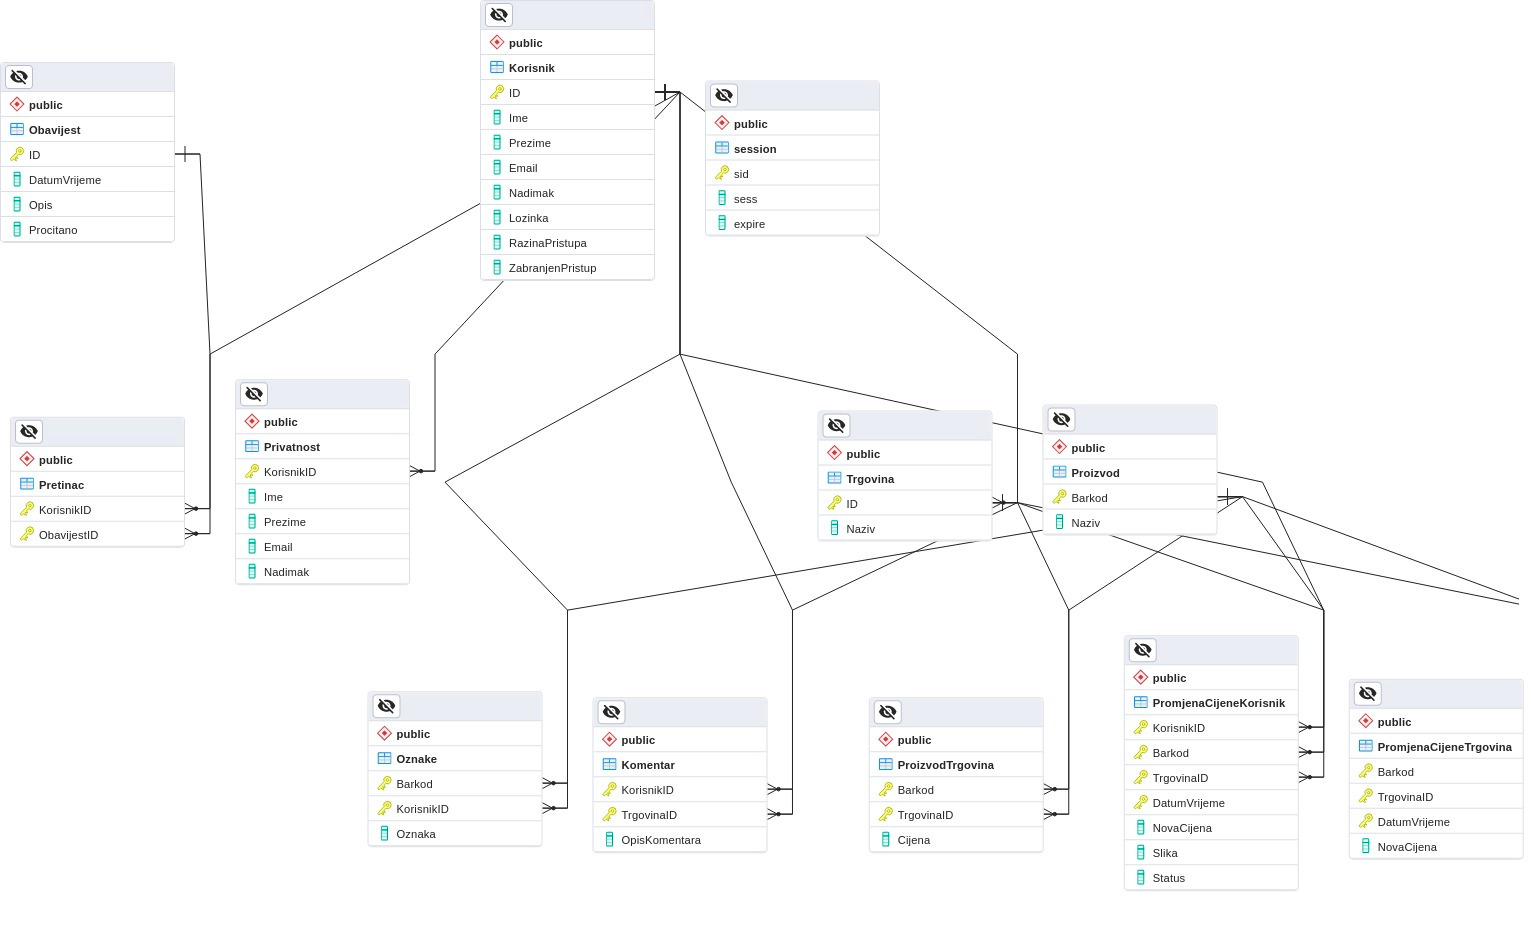
\includegraphics[width=\textwidth]{slike/ERDijagramBaza.JPEG} %veličina u odnosu na širinu linije
			\caption{E-R Dijagram baze podataka}
			\label{fig:ERDijagramBaza} %label mora biti drugaciji za svaku sliku
			\end{figure}
			
			\eject
			
			
		\section{Dijagram razreda}
		
			%\textit{Potrebno je priložiti dijagram razreda s pripadajućim opisom. Zbog preglednosti je moguće dijagram razlomiti na više njih, ali moraju biti grupirani prema sličnim razinama apstrakcije i srodnim funkcionalnostima.}\\
			\textbf{UserModel} služi za spremanje podataka o korisniku te za autentifikaciju i autorizaciju korisnika. 
			\textbf{UserModel} generalizira \textbf{Admin} i \textbf{StoreModel}.
			 
			\textbf{PrivacyModel} pohranjuje podatke o tome koji će podaci o korisniku biti javni, a koji privatni.
			  
			\textbf{Admin} sadrži metode koje može izvršiti isključivo korisnik s admin pravom pristupa(odobravanje promjena cijena, zabrana pristupa drugim korisnicima...) 
			
			\textbf{StoreModel} modelira trgovinu. 
			
			\textbf{ProductModel} modelira proizvod. Proizvod je jednoznačno određen barkodom kako bi više trgovina moglo imati isti proizvod u ponudi. 
			
			\textbf{PriceChangeLog} služi za opisivanje promjena cijena proizvoda u nekoj trgovini u nekom vremenskom razdoblju. 
			
			\textbf{PriceChangeRequestModel} modelira zahtjev za promjenom cijene koje šalje korisnik za proizvod u nekoj trgovini u kojoj se stvarna cijena razlikuje od cijene navedene u aplikaciji.  
			
			\textbf{NotificationModel} modelira obavijesti koje admin može slati korisniku ili trgovini.
Klase iz data access paketa sadržavaju isključivo statičke metode koje služe za komunikaciju s bazom podataka.

\begin{figure}[H]
			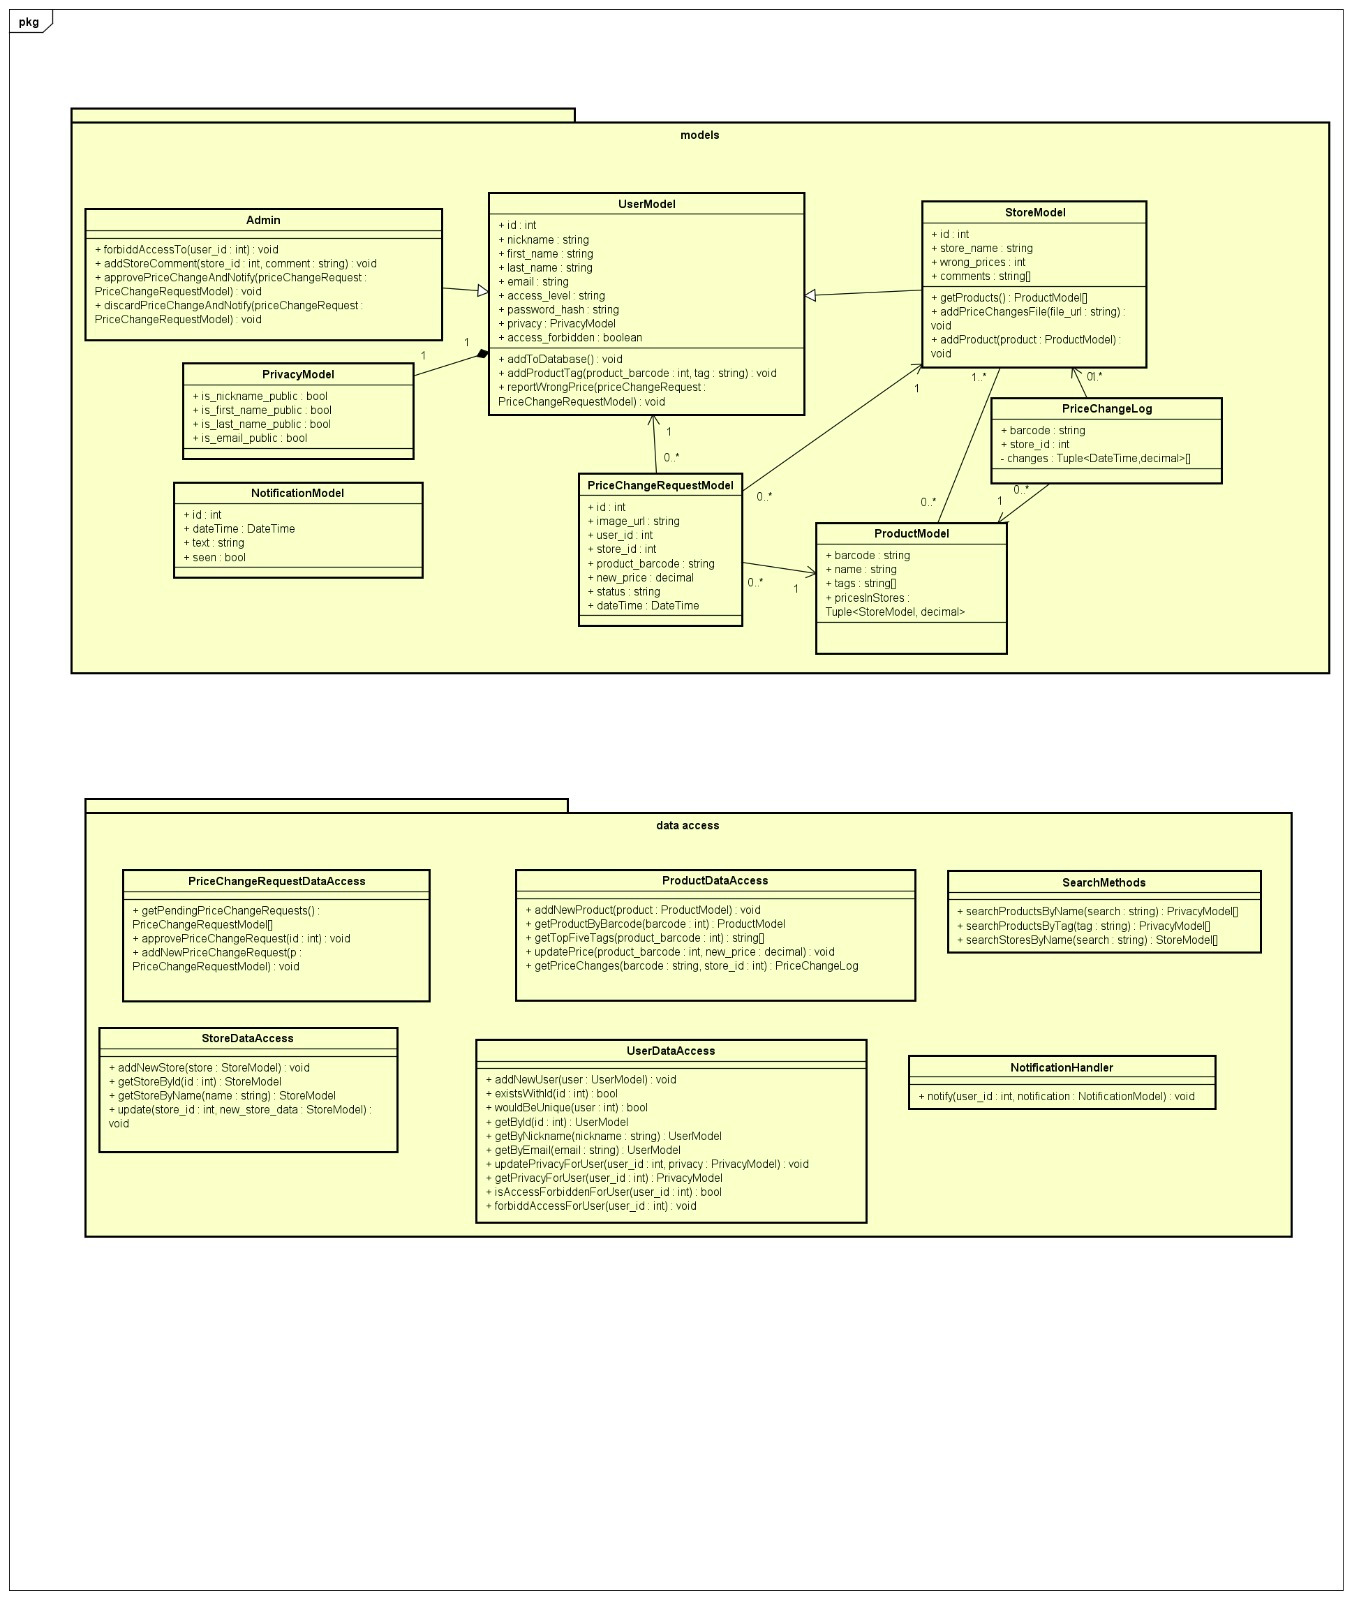
\includegraphics[width=\textwidth]{slike/dijagramRazreda.png} %veličina u odnosu na širinu linije
			\caption{dijagram razreda}
			\label{fig:dijagramRazreda} %label mora biti drugaciji za svaku sliku
			\end{figure}
			
			%\textbf{\textit{dio 1. revizije}}\\
			
			%\textit{Prilikom prve predaje projekta, potrebno je priložiti potpuno razrađen dijagram razreda vezan uz \textbf{generičku funkcionalnost} sustava. Ostale funkcionalnosti trebaju biti idejno razrađene u dijagramu sa sljedećim komponentama: nazivi razreda, nazivi metoda i vrste pristupa metodama (npr. javni, zaštićeni), nazivi atributa razreda, veze i odnosi između razreda.}\\
			
			%\textbf{\textit{dio 2. revizije}}\\			
			
			%\textit{Prilikom druge predaje projekta dijagram razreda i opisi moraju odgovarati stvarnom stanju implementacije}
			
			
			
			\eject
		
		%\section{Dijagram stanja}
			
			
			%\textbf{\textit{dio 2. revizije}}\\
			
			%\textit{Potrebno je priložiti dijagram stanja i opisati ga. Dovoljan je jedan dijagram stanja koji prikazuje \textbf{značajan dio funkcionalnosti} sustava. Na primjer, stanja korisničkog sučelja i tijek korištenja neke ključne funkcionalnosti jesu značajan dio sustava, a registracija i prijava nisu. }
			
			
			%\eject 
		
		%\section{Dijagram aktivnosti}
			
			%\textbf{\textit{dio 2. revizije}}\\
			
			% \textit{Potrebno je priložiti dijagram aktivnosti s pripadajućim opisom. Dijagram aktivnosti treba prikazivati značajan dio sustava.}
			
		%	\eject
		%\section{Dijagram komponenti}
		
			%\textbf{\textit{dio 2. revizije}}\\
		
			% \textit{Potrebno je priložiti dijagram komponenti s pripadajućim opisom. Dijagram komponenti treba prikazivati strukturu cijele aplikacije.}
	\chapter{Implementacija i korisničko sučelje}
		
		
		\section{Korištene tehnologije i alati}
		
			%\textbf{\textit{dio 2. revizije}}
			
			% \textit{Detaljno navesti sve tehnologije i alate koji su primijenjeni pri izradi dokumentacije i aplikacije. Ukratko ih opisati, te navesti njihovo značenje i mjesto primjene. Za svaki navedeni alat i tehnologiju je potrebno \textbf{navesti internet poveznicu} gdje se mogu preuzeti ili više saznati o njima}.
			Za izradu dokumentacije korišten je alat \textbf{Texmaker} koji je razvojna okolina za jezik \textbf{LaTex}. \textit{LaTex} je programski jezik za pisanje strukturiranih tekstova. Najčešće se koristi u oblikovanju znanstvenih radova.
			
			Dijagrami unutar dokumentacije izrađeni su pomoću alata \textbf{Astah UML} i \textbf{lucid.app}. \textit{Astah UML} aplikacija je za modeliranje UML-a. \textit{Lucid.app} je web-stranica koja nudi isto to, no pristupačnija jer se ne mora preuzimati. Obje aplikacije se za studente ne naplaćuju.
			
			Komunikacija tima odvijala se preko aplikacije \textbf{WhatsApp}. Za potrebe ovog projekta bila je sasvim dovoljna, no za neke ozbiljnije projekte bilo bi potrebno prijeći na bolji alat.
			
			Kao sustav za upravljanje izvornim kodom korišten je \textbf{Git}. Udaljeni repozitorij projekta je dostupan na web platformi \textbf{GitLab}.
			
			Aplikacija je napisana u \textbf{Express}-u, framework za izgradnju web-aplikacija na platformi \textbf{node.js}. Sve to je ostvareno programskim jezikom \textbf{Javascript}. \textit{Node.js} je back-end JavaScript runtime okruženje, radi na V8 JavaScript Engineu i izvršava JavaScript kod izvan web preglednika. 
			
			Baza podataka je 
			
			\eject 
		
	
		\section{Ispitivanje programskog rješenja}
			
			\textbf{\textit{dio 2. revizije}}\\
			
			 \textit{U ovom poglavlju je potrebno opisati provedbu ispitivanja implementiranih funkcionalnosti na razini komponenti i na razini cijelog sustava s prikazom odabranih ispitnih slučajeva. Studenti trebaju ispitati temeljnu funkcionalnost i rubne uvjete.}
	
			
			\subsection{Ispitivanje komponenti}
			\textit{Potrebno je provesti ispitivanje jedinica (engl. unit testing) nad razredima koji implementiraju temeljne funkcionalnosti. Razraditi \textbf{minimalno 6 ispitnih slučajeva} u kojima će se ispitati redovni slučajevi, rubni uvjeti te izazivanje pogreške (engl. exception throwing). Poželjno je stvoriti i ispitni slučaj koji koristi funkcionalnosti koje nisu implementirane. Potrebno je priložiti izvorni kôd svih ispitnih slučajeva te prikaz rezultata izvođenja ispita u razvojnom okruženju (prolaz/pad ispita). }
			
			
			
			\subsection{Ispitivanje sustava}
			
			 \textit{Potrebno je provesti i opisati ispitivanje sustava koristeći radni okvir Selenium\footnote{\url{https://www.seleniumhq.org/}}. Razraditi \textbf{minimalno 4 ispitna slučaja} u kojima će se ispitati redovni slučajevi, rubni uvjeti te poziv funkcionalnosti koja nije implementirana/izaziva pogrešku kako bi se vidjelo na koji način sustav reagira kada nešto nije u potpunosti ostvareno. Ispitni slučaj se treba sastojati od ulaza (npr. korisničko ime i lozinka), očekivanog izlaza ili rezultata, koraka ispitivanja i dobivenog izlaza ili rezultata.\\ }
			 
			 \textit{Izradu ispitnih slučajeva pomoću radnog okvira Selenium moguće je provesti pomoću jednog od sljedeća dva alata:}
			 \begin{itemize}
			 	\item \textit{dodatak za preglednik \textbf{Selenium IDE} - snimanje korisnikovih akcija radi automatskog ponavljanja ispita	}
			 	\item \textit{\textbf{Selenium WebDriver} - podrška za pisanje ispita u jezicima Java, C\#, PHP koristeći posebno programsko sučelje.}
			 \end{itemize}
		 	\textit{Detalji o korištenju alata Selenium bit će prikazani na posebnom predavanju tijekom semestra.}
			
			\eject 
		
		
		%\section{Dijagram razmještaja}
			
			\textbf{\textit{dio 2. revizije}}
			
			 \textit{Potrebno je umetnuti \textbf{specifikacijski} dijagram razmještaja i opisati ga. Moguće je umjesto specifikacijskog dijagrama razmještaja umetnuti dijagram razmještaja instanci, pod uvjetom da taj dijagram bolje opisuje neki važniji dio sustava.}
			
			\eject 
		
		\section{Upute za puštanje u pogon}
		
			\textbf{\textit{dio 2. revizije}}\\
		
			 \textit{U ovom poglavlju potrebno je dati upute za puštanje u pogon (engl. deployment) ostvarene aplikacije. Na primjer, za web aplikacije, opisati postupak kojim se od izvornog kôda dolazi do potpuno postavljene baze podataka i poslužitelja koji odgovara na upite korisnika. Za mobilnu aplikaciju, postupak kojim se aplikacija izgradi, te postavi na neku od trgovina. Za stolnu (engl. desktop) aplikaciju, postupak kojim se aplikacija instalira na računalo. Ukoliko mobilne i stolne aplikacije komuniciraju s poslužiteljem i/ili bazom podataka, opisati i postupak njihovog postavljanja. Pri izradi uputa preporučuje se \textbf{naglasiti korake instalacije uporabom natuknica} te koristiti što je više moguće \textbf{slike ekrana} (engl. screenshots) kako bi upute bile jasne i jednostavne za slijediti.}
			
			
			 \textit{Dovršenu aplikaciju potrebno je pokrenuti na javno dostupnom poslužitelju. Studentima se preporuča korištenje neke od sljedećih besplatnih usluga: \href{https://aws.amazon.com/}{Amazon AWS}, \href{https://azure.microsoft.com/en-us/}{Microsoft Azure} ili \href{https://www.heroku.com/}{Heroku}. Mobilne aplikacije trebaju biti objavljene na F-Droid, Google Play ili Amazon App trgovini.}
			
			
			\eject 
	\chapter{Zaključak i budući rad}
		
		\textbf{\textit{dio 2. revizije}}\\
		
		 \textit{U ovom poglavlju potrebno je napisati osvrt na vrijeme izrade projektnog zadatka, koji su tehnički izazovi prepoznati, jesu li riješeni ili kako bi mogli biti riješeni, koja su znanja stečena pri izradi projekta, koja bi znanja bila posebno potrebna za brže i kvalitetnije ostvarenje projekta i koje bi bile perspektive za nastavak rada u projektnoj grupi.}
		
		 \textit{Potrebno je točno popisati funkcionalnosti koje nisu implementirane u ostvarenoj aplikaciji.}
		
		\eject 
	\chapter*{Popis literature}
		\addcontentsline{toc}{chapter}{Popis literature}
	 	
 		\textbf{\textit{Kontinuirano osvježavanje}}
	
		\textit{Popisati sve reference i literaturu koja je pomogla pri ostvarivanju projekta.}
		
		
		\begin{enumerate}
			
			
			\item  Programsko inženjerstvo, FER ZEMRIS, \url{http://www.fer.hr/predmet/proinz}
			
			\item  I. Sommerville, "Software engineering", 8th ed, Addison Wesley, 2007.
			
			\item  T.C.Lethbridge, R.Langaniere, "Object-Oriented Software Engineering", 2nd ed. McGraw-Hill, 2005.
			
			\item  I. Marsic, Software engineering book``, Department of Electrical and Computer Engineering, Rutgers University, \url{http://www.ece.rutgers.edu/~marsic/books/SE}
			
			\item  The Unified Modeling Language, \url{https://www.uml-diagrams.org/}
			
			\item  Astah Community, \url{http://astah.net/editions/uml-new}
			\item Lucid.app, \url{https://lucid.app/}
			\item Pgadmin, \url{https://www.pgadmin.org/}
		\end{enumerate}
		
		
		 
	
	
	\begingroup
	\renewcommand*\listfigurename{Indeks slika i dijagrama}
	%\renewcommand*\listtablename{Indeks tablica}
	%\let\clearpage\relax
	\listoffigures
	%\vspace{10mm}
	%\listoftables
	\endgroup
	\addcontentsline{toc}{chapter}{Indeks slika i dijagrama}


	
	\eject 
		
	\chapter*{Dodatak: Prikaz aktivnosti grupe}
		\addcontentsline{toc}{chapter}{Dodatak: Prikaz aktivnosti grupe}
		
		\section*{Dnevnik sastajanja}
		
		%\textbf{\textit{Kontinuirano osvježavanje}}\\
		
		% \textit{U ovom dijelu potrebno je redovito osvježavati dnevnik sastajanja prema predlošku.}
		
		\begin{packed_enum}
			\item  sastanak
			
			\item[] \begin{packed_item}
				\item Datum: u ovom formatu: 20.10.2022.
				\item Prisustvovali: J.Vrsalović, V.Krušić, A.Macan, P.Novak, V.Perković, L.Vrsalović, L.Zekan
				\item Teme sastanka:
				\begin{packed_item}
					\item  ideje o dodijeljenoj temi
					\item  raspodjela uloga u timu
				\end{packed_item}
			\end{packed_item}
			
			\item  sastanak
			\item[] \begin{packed_item}
				\item Datum: u ovom formatu: 26.10.2022.
				\item Prisustvovali: L.Vrsalović, V.Perković
				\item Teme sastanka:
				\begin{packed_item}
					\item  Podjela posla u dokumentaciji
					\item  Instalacija i pokretanje alata
				\end{packed_item}
			\end{packed_item}
			
			\item  sastanak
			\item[] \begin{packed_item}
				\item Datum: u ovom formatu: 2.11.2022.
				\item Prisustvovali: J.Vrsalović, Petar Novak, Anton Macan
				\item Teme sastanka:
				\begin{packed_item}
					\item  Back end
					\item  Koncept baze podataka
				\end{packed_item}
			\end{packed_item}
			
			\item  sastanak
			\item[] \begin{packed_item}
				\item Datum: u ovom formatu: 3.11.2022.
				\item Prisustvovali: J.Vrsalović, V.Krušić, L.Zekan
				\item Teme sastanka:
				\begin{packed_item}
					\item  Login forma
					\item  Homepage
				\end{packed_item}
			\end{packed_item}
			
			
			%
			
		\end{packed_enum}
		
		\eject
		\section*{Tablica aktivnosti}
		
			%\textbf{\textit{Kontinuirano osvježavanje}}\\
			
			% \textit{Napomena: Doprinose u aktivnostima treba navesti u satima po članovima grupe po aktivnosti.}

			\begin{longtblr}[
					label=none,
				]{
					vlines,hlines,
					width = \textwidth,
					colspec={X[7, l]X[1, c]X[1, c]X[1, c]X[1, c]X[1, c]X[1, c]X[1, c]}, 
					vline{1} = {1}{text=\clap{}},
					hline{1} = {1}{text=\clap{}},
					rowhead = 1,
				} 
				\multicolumn{1}{c|}{} & \multicolumn{1}{c|}{\rotatebox{90}{\textbf{Joško Vrsalović}}} & \multicolumn{1}{c|}{\rotatebox{90}{\textbf{Vida Krušić}}} &	\multicolumn{1}{c|}{\rotatebox{90}{\textbf{Anton Macan }}} & \multicolumn{1}{c|}{\rotatebox{90}{\textbf{Petar Novak }}} &	\multicolumn{1}{c|}{\rotatebox{90}{\textbf{Vlado Perković }}} & \multicolumn{1}{c|}{\rotatebox{90}{\textbf{Lovro Vrsalović }}} &	\multicolumn{1}{c|}{\rotatebox{90}{\textbf{Luka Zekan }}} \\  
				Upravljanje projektom 		& 8 &  &  &  &  &  & \\ 
				Opis projektnog zadatka 	&  &  &  &  & 4 &  & \\ 
				
				Funkcionalni zahtjevi       &  &  &  &  &  & 1 &  \\ 
				Opis pojedinih obrazaca 	&  &  &  &  & 1 & 4 &  \\ 
				Dijagram obrazaca 			&  &  &  &  &  & 3 &  \\ 
				Sekvencijski dijagrami 		&  &  &  &  & 2 &  &  \\ 
				Opis ostalih zahtjeva 		&  &  &  &  &  & 1 &  \\ 

				Arhitektura i dizajn sustava	 &  &  &  &  &  &  & 3 \\ 
				Baza podataka				&  &  & 4 &  &  &  &   \\ 
				Dijagram razreda 			&  &  &  & 5 &  &  &   \\ 
				Dijagram stanja				&  &  &  &  &  &  &  \\ 
				Dijagram aktivnosti 		&  &  &  &  &  &  &  \\ 
				Dijagram komponenti			&  &  &  &  & 4 &  &  \\ 
				Korištene tehnologije i alati 		&  &  &  &  & 2 &  &  \\ 
				Ispitivanje programskog rješenja 	&  &  &  &  &  &  &  \\ 
				Dijagram razmještaja			&  &  &  &  & 2 &  &  \\ 
				Upute za puštanje u pogon 		&  &  &  &  &  &  &  \\  
				Dnevnik sastajanja 			&  &  &  &  & 1 &  &  \\ 
				Zaključak i budući rad 		&  &  &  &  &  &  &  \\  
				Popis literature 			&  &  &  &  & 1 &  &  \\  
				&  &  &  &  &  &  &  \\ \hline 
				\textit{homepage} 			&  & 4 &  &  &  &  & 1 \\ 
				\textit{forme za login i signup} 				&  & 2 &  &  &  &  &  \\  
				\textit{izrada baze podataka} 		 			&  &  & 4 &  &  &  & \\  
				\textit{spajanje s bazom podataka} 							&  &  &  & 4 &  &  &  \\ 
				\textit{back end} 							& 2 &  &  & 5 &  &  &  \\  
				\textit{deployment} 			& 5 &  &  &  &  &  &  \\
			\end{longtblr}
					
					
		\eject
		\section*{Dijagrami pregleda promjena}
		
		\textbf{\textit{dio 2. revizije}}\\
		
		\textit{Prenijeti dijagram pregleda promjena nad datotekama projekta. Potrebno je na kraju projekta generirane grafove s gitlaba prenijeti u ovo poglavlje dokumentacije. Dijagrami za vlastiti projekt se mogu preuzeti s gitlab.com stranice, u izborniku Repository, pritiskom na stavku Contributors.}
		
	


\end{document} %naredbe i tekst nakon ove naredbe ne ulaze u izgrađen dokument 


